% pyformex manual --- examples
% $Id$
% (C) B.Verhegghe

\chapter{pyFormex example scripts}
\label{cha:examples}

\section{Creating geometry}
\label{sec:creating-geometry}

To explain the modus operandi of \pyf, the \file{WireStent.py} script is parsed step by step. To start, all required modules to run the \file{WireStent.py} script are imported (e.g. the \code{math} module to use the mathematical constant $\pi$). Subsequently, the class \code{DoubleHelixStent} is defined which allows the simple use of the geometrical model in other scripts for e.g. parametric, optimization and finite element analyses of braided wire stents. Consequently, the latter scripts do not have to contain the wire stent geometry building and can be condensed and conveniently arranged. The definition of the class starts with a $"""$documentation string$"""$, explaining its aim and functioning.

\verbatiminput{scripts/WireStent1.py}

The constructor \code{\_\_init\_\_} of the \code{DoubleHelixStent} class requires 8 arguments:
\begin{itemize}
\item stent external diameter $De$ (\unit{mm}).
\item stent length $L$ (\unit{mm}).
\item wire diameter $d$ (\unit{mm}).
\item Number of wires in one spiral set, i.e. wires with the same orientation, $nx$ (\unit{-}).
\item Pitch angle $\beta$ (\unit{$\deg$}).
\item Extra radial distance between the crossing wires $ds$ (\unit{mm}). By default, $ds$ is \unit[0.0]{mm} for crossing wires, corresponding with a centre line distance between two crossing wires of exactly $d$.
\item Number of elements in a strut, i.e. part of a wire between two crossings, $nb$ (\unit{-}). As every base element is a straight line, multiple elements are required to approximate the curvature of the stent wires. The default value of 4 elements in a strut is a good assumption.
\item If \code{connectors=True}, extra elements are created at the positions where there is physical contact between the crossing wires. These elements are required to enable contact between these wires in finite element analyses.
\end{itemize}

The virtual construction of the wire stent structure is defined by the following sequence of four operations: (i) Creation of a nearly planar base module of two crossing wires; (ii) Extending the base module with a mirrored and translated copy; (iii) Replicating the extended base module in both directions of the base plane; and (iv) Rolling the nearly planar grid into the cylindrical stent structure, which is easily parametric adaptable.

\subsection{Creating the base module}

Depending on the specified arguments in the constructor, the mean stent diameter $D$, the average stent radius $r$, the \code{bump} or curvature of the wires $dz$, the pitch $p$ and the number of base modules in the axial direction $ny$ are calculated with the following script. As the wire stent structure is obtained by braiding, the wires have an undulating course and the \code{bump dz} corresponds to the amplitude of the wave. If no extra distance $ds$ is specified, there will be exactly one wire diameter between the centre lines of the crossing wires. The number of modules in the axial direction $ny$ is an integer, therefore, the actual length of the stent model might differ slightly from the specified, desired length $L$. However, this difference has a negligible impact on the numerical results.

\verbatiminput{scripts/WireStent2.py}

Of now, all parameters to describe the stent geometry are specified and available to start the construction of the wire stent. Initially a simple Formex is created using the \code{pattern()}-function: a straigth line segment of length 1 oriented along the X-axis (East or $1$-direction). The \code{replic()}-functionality replicates this line segment $nb$ times with step {1} in the X-direction ($0$-direction). Subsequently, these $nb$ line segments form a new Formex which is given a one-dimensional \code{bump} with the \code{bump1()}-function. The Formex undergoes a deformation in the Z-direction ($2$-direction), forced by the point \code{[0,0,dz]}. The \code{bump} intensity is specified by the quadratic \code{bump\_z} function and varies along the X-axis ($0$-axis). The creation of this single bumped strut, oriented along the X-axis is summarized in the next script and depicted in Figure \ref{bumped}.

\verbatiminput{scripts/WireStent3.py}

\begin{figure} [ht]
   \centering
   \begin{makeimage}
   \end{makeimage}
   \begin{latexonly}
	\hspace{0.1cm}
	\begin{minipage} [c] [] [c]{3.5cm} 
	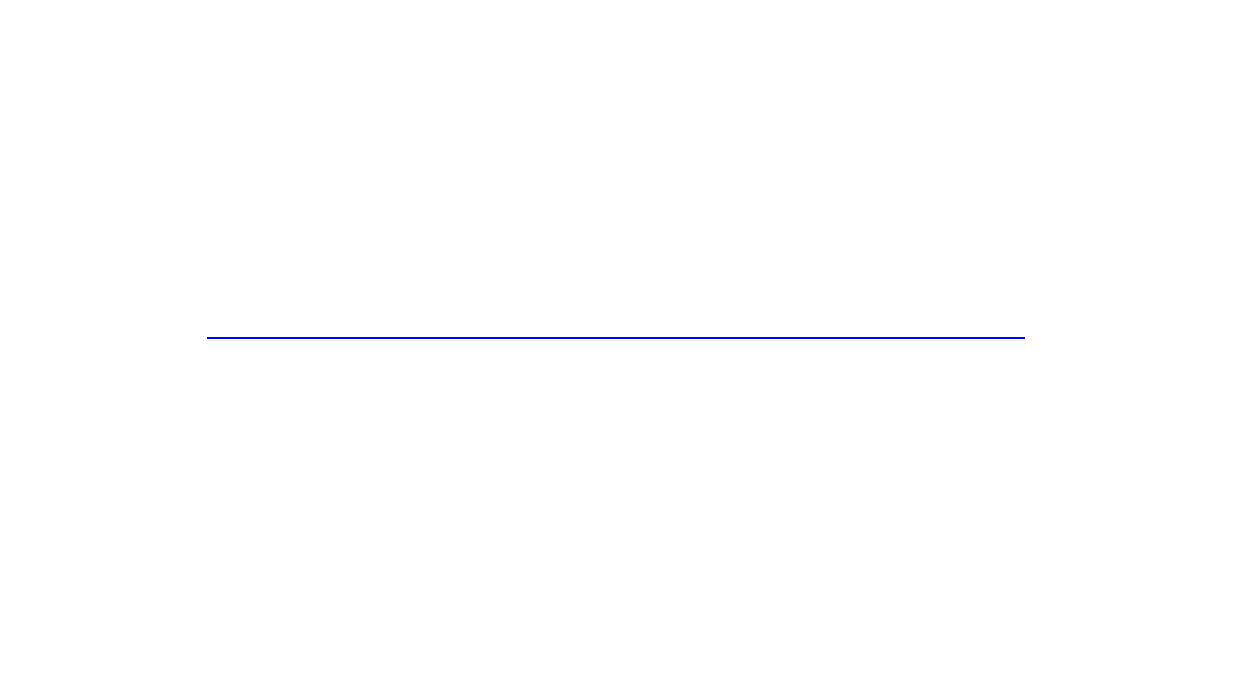
\includegraphics [width =\textwidth] {images/WireStentDemot2Step01}
	\begin{center}
	\vspace{-3ex}
	(a)
	\vspace{1ex}
	\end{center}
\end{minipage}
\hspace{0.3cm}
\begin{minipage} [c] [] [c] {3.5cm}
	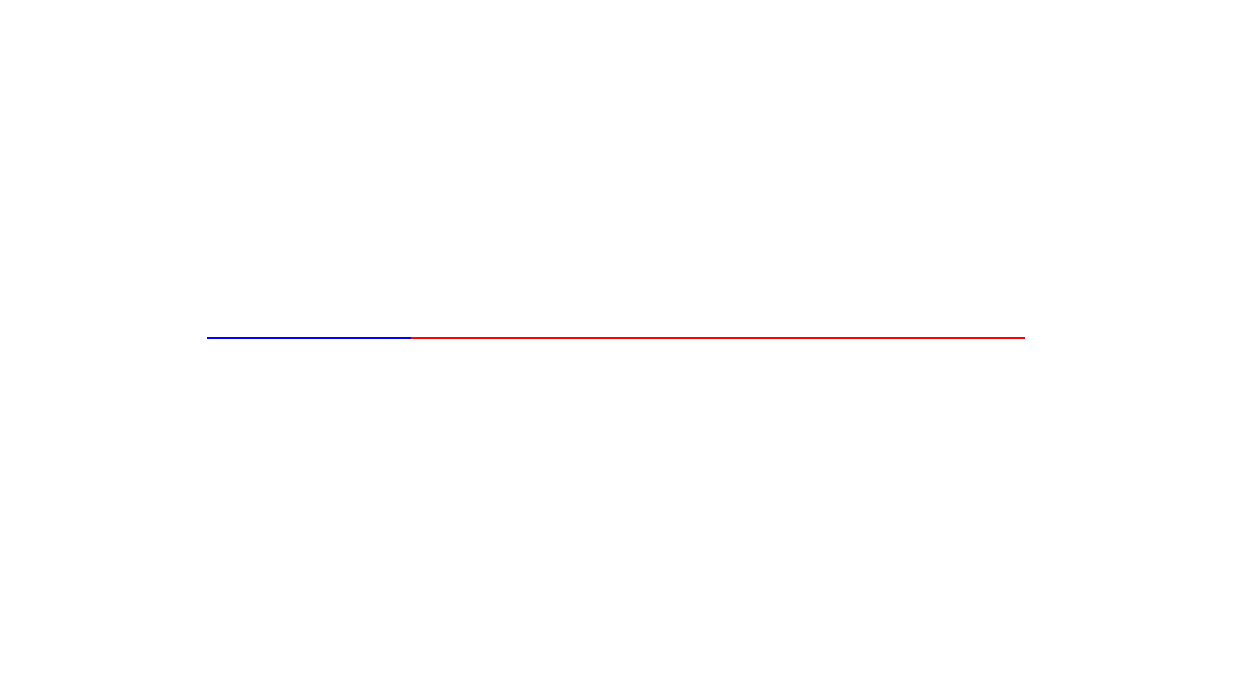
\includegraphics [width =\textwidth] {images/WireStentDemot2Step02}
	\begin{center}
	\vspace{-3ex}
	(b)
	\vspace{1ex}
	\end{center}
\end{minipage}
\hspace{0.3cm}
\begin{minipage} [c] [] [c] {3.5cm}
	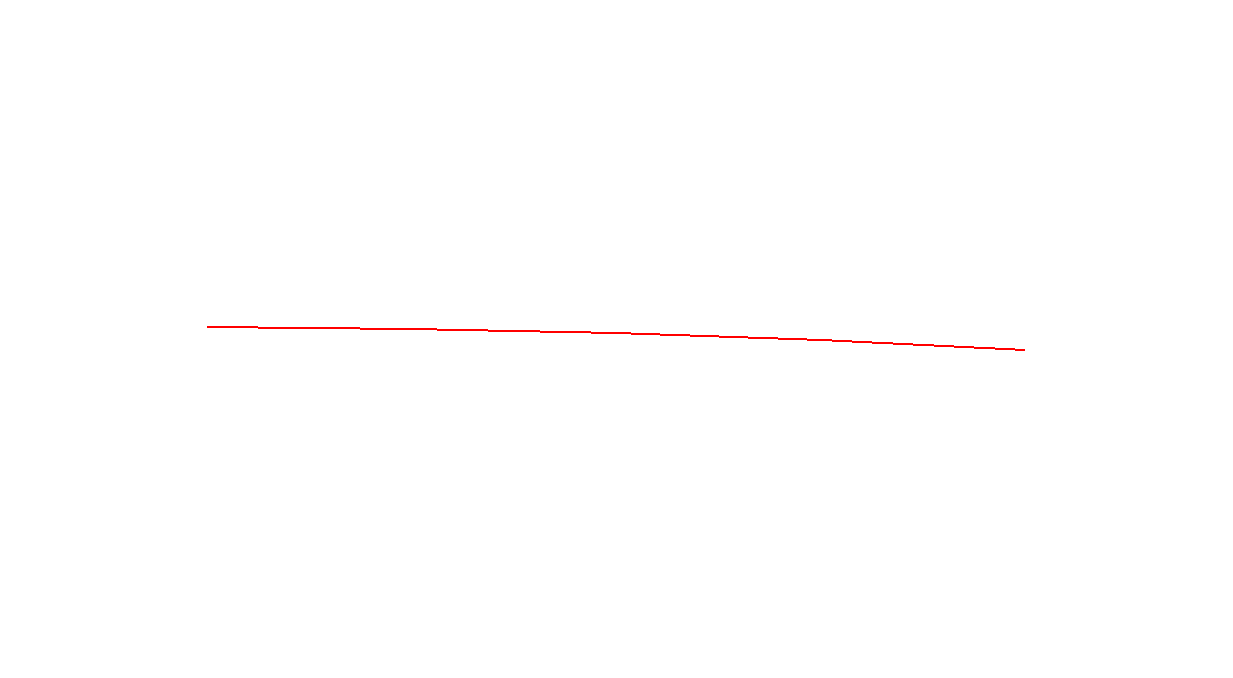
\includegraphics [width =\textwidth] {images/WireStentDemot2Step03}
	\begin{center}
	\vspace{-3ex}
	(c)
	\vspace{1ex}
	\end{center}
\end{minipage}
\hspace{0.3cm}	
   \end{latexonly}
   \begin{htmlonly}
     \htmladdimg{../images/WireStentDemot2Step01.png}
     \htmladdimg{../images/WireStentDemot2Step02.png}
     \htmladdimg{../images/WireStentDemot2Step03.png}
   \end{htmlonly}

	\caption {Creation of single bumped strut (c) from a straight (a) and replicated (b) line segment.} 
	\label{bumped}	
\end{figure}

The single bumped strut (\code{base}) is rescaled homothetically in the XY-plane to size one with the \code{scale()}-function. Subsequently, the \code{shear()}-functionality generates a new \code{NE} Formex by skewing the \code{base} Formex in the Y-direction ($1$-direction) with a \code{skew} factor of $1$ in the YX-plane. As a result, the Y-coordinates of the \code{base} Formex are altered according to the following rule: $y_2 = y_1 + skew * x_1$. Similarly a \code{SE} Formex is generated by a \code{shear()} operation on a mirrored copy of the \code{base} Formex. The \code{base} copy, mirrored in the direction of the XY-plane (perpendicular to the $2$-axis), is obtained by the \code{reflect()} command. Both Formices are given a different property number by the \code{setProp()}-function, visualised by the different color codes in Figure \ref{base} This number can be used as an entry in a database, which holds some sort of property. The Formex and the database are two seperate entities, only linked by the property numbers. The \code{rosette()}-function creates a unit cell of crossing struts by $2$ rotational replications with an angular step of \unit[180]{$\deg$} around the Z-axis (the original Formex is the first of the $2$ replicas). If specified in the constructor, an additional Formex with property $2$ connects the first points of the \code{NE} and \code{SE} Formices.
%
\verbatiminput{scripts/WireStent4.py}

\begin{figure} [ht]
   \centering
   \begin{makeimage}
   \end{makeimage}
   \begin{latexonly}
	\hspace{0.1cm}
	\begin{minipage} [c] [] [c]{3.5cm} 
	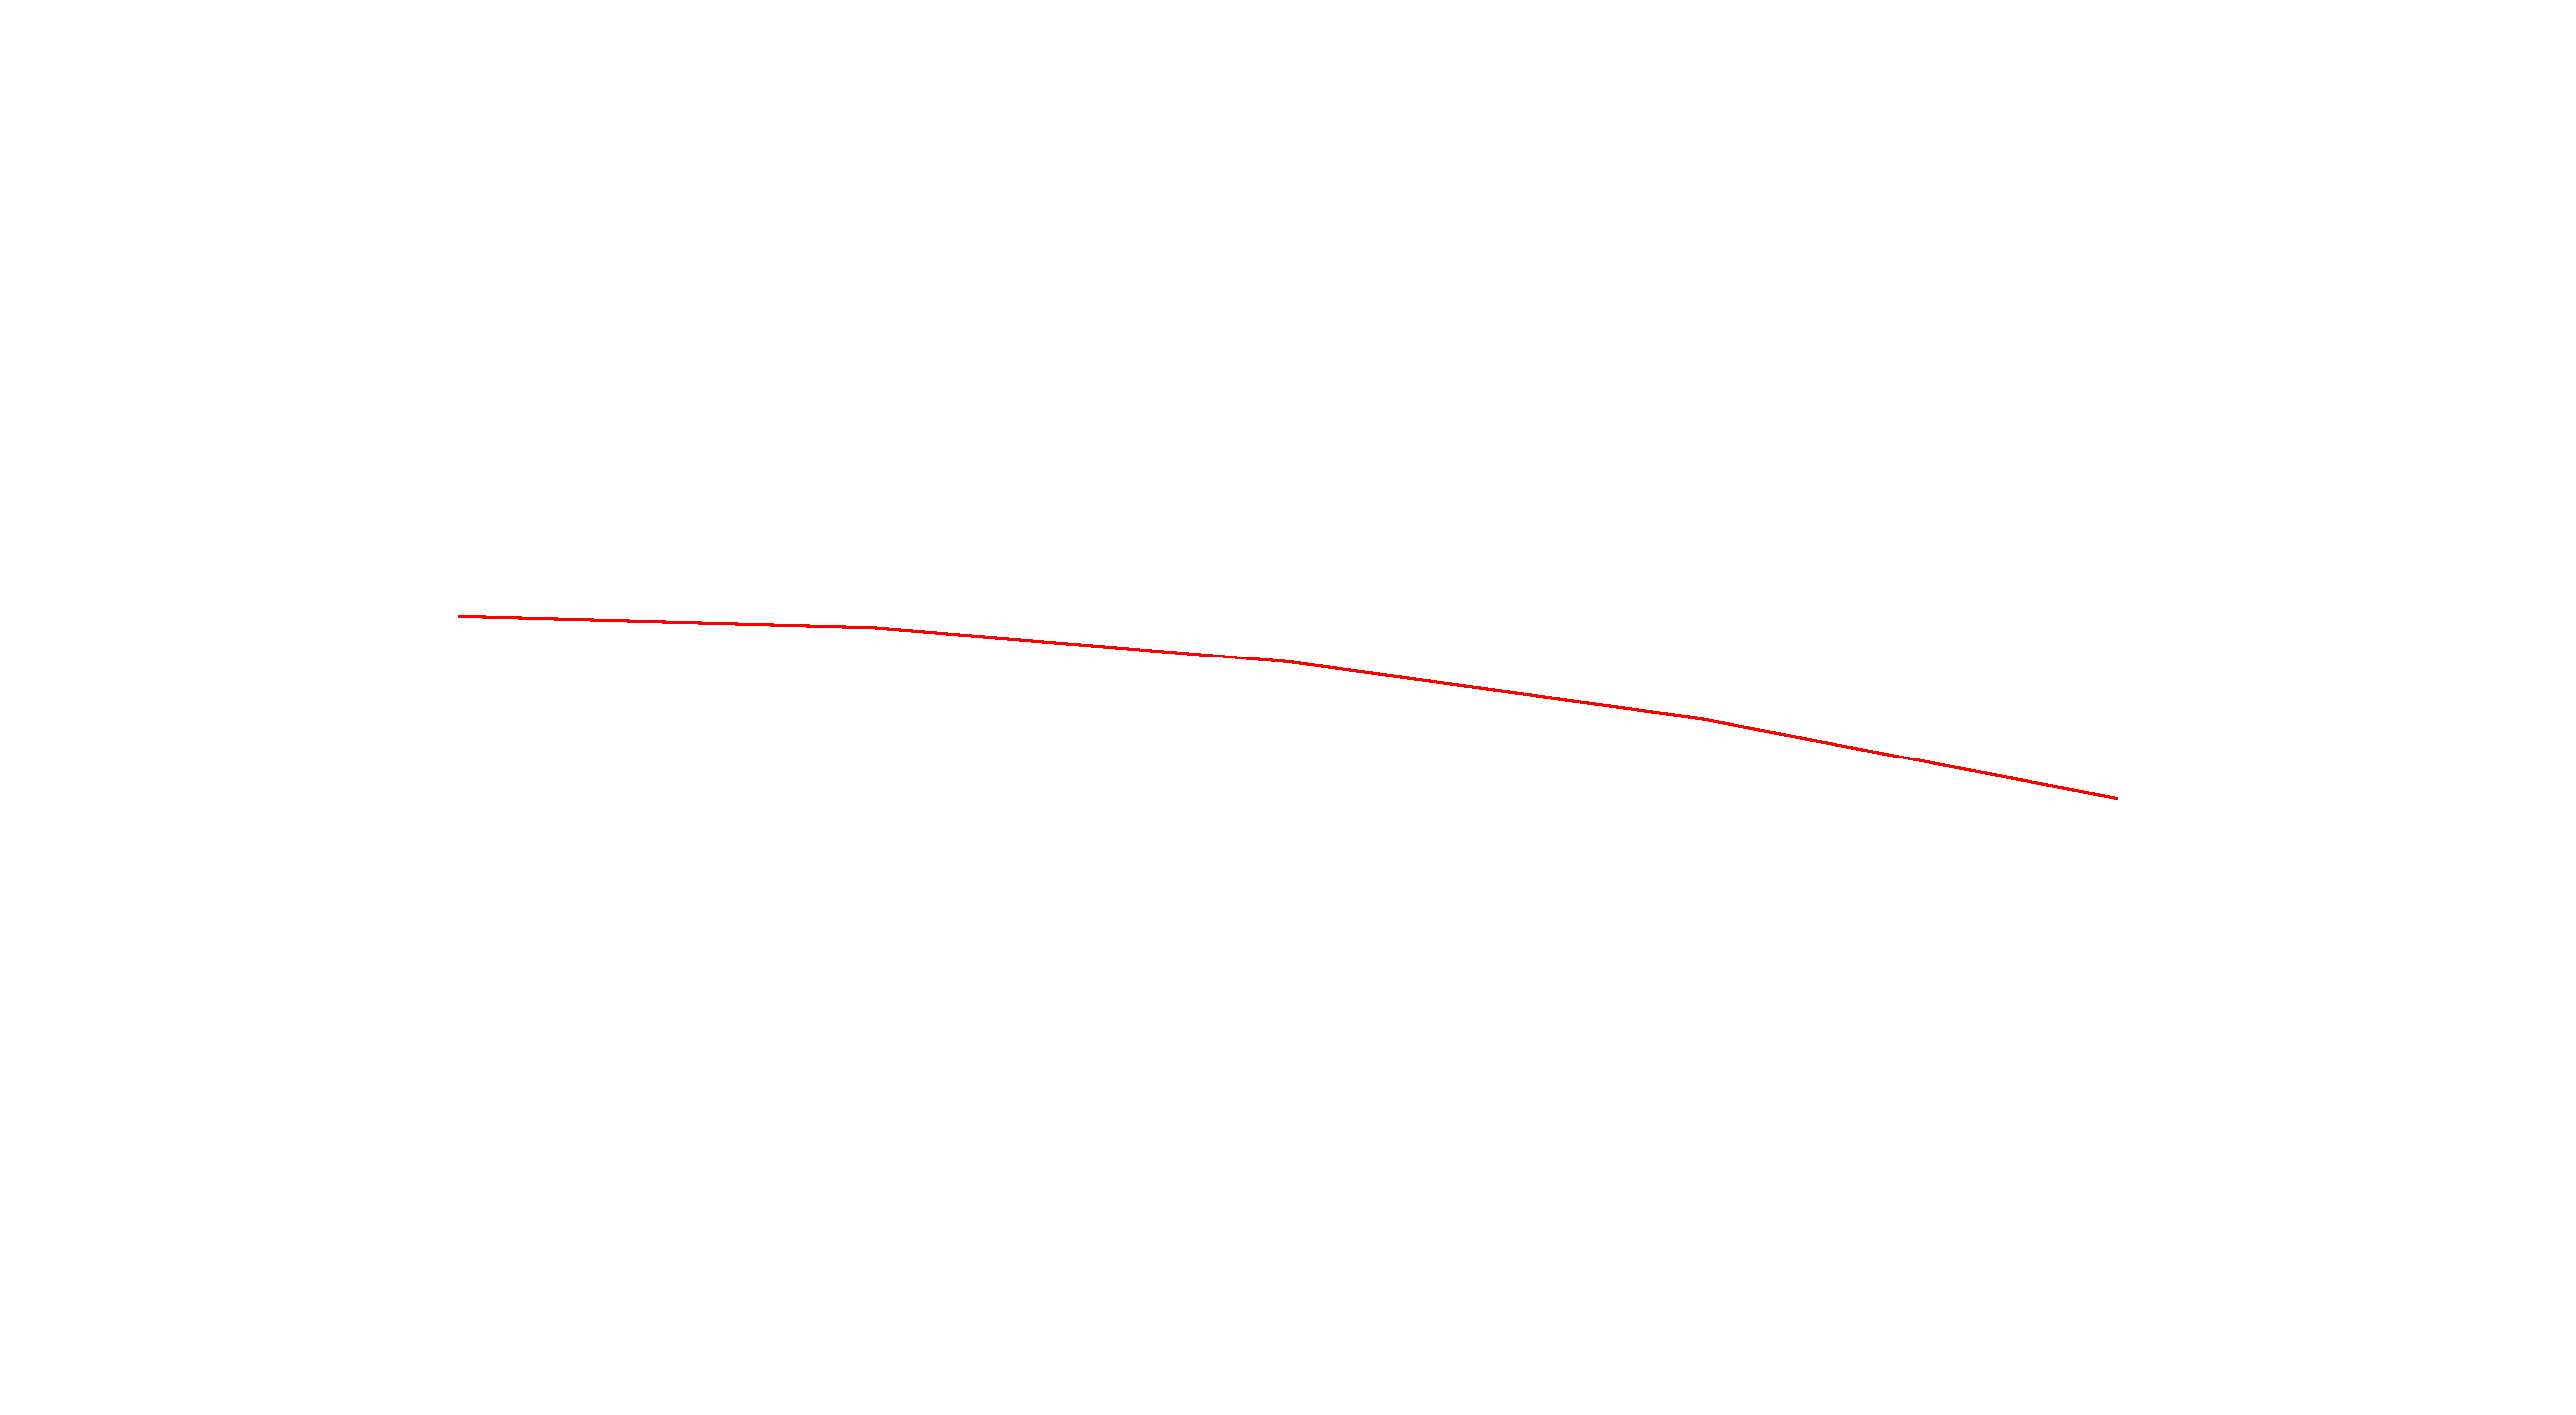
\includegraphics [width =\textwidth] {images/WireStentDemot2Step04}
	\begin{center}
	\vspace{-3ex}
	(a)
	\vspace{1ex}
	\end{center}
\end{minipage}
\hspace{0.3cm}
\begin{minipage} [c] [] [c] {3.5cm}
	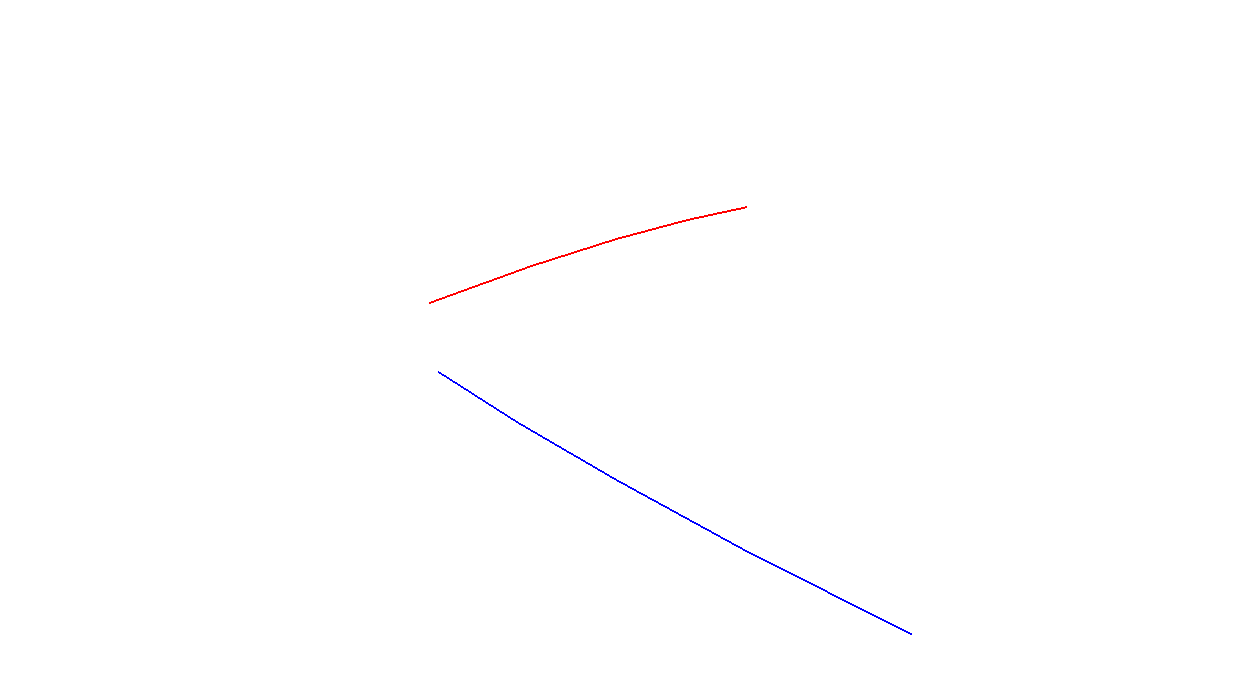
\includegraphics [width =\textwidth] {images/WireStentDemot2Step07}
	\begin{center}
	\vspace{-3ex}
	(b)
	\vspace{1ex}
	\end{center}
\end{minipage}
\hspace{0.3cm}
\begin{minipage} [c] [] [c] {3.5cm}
	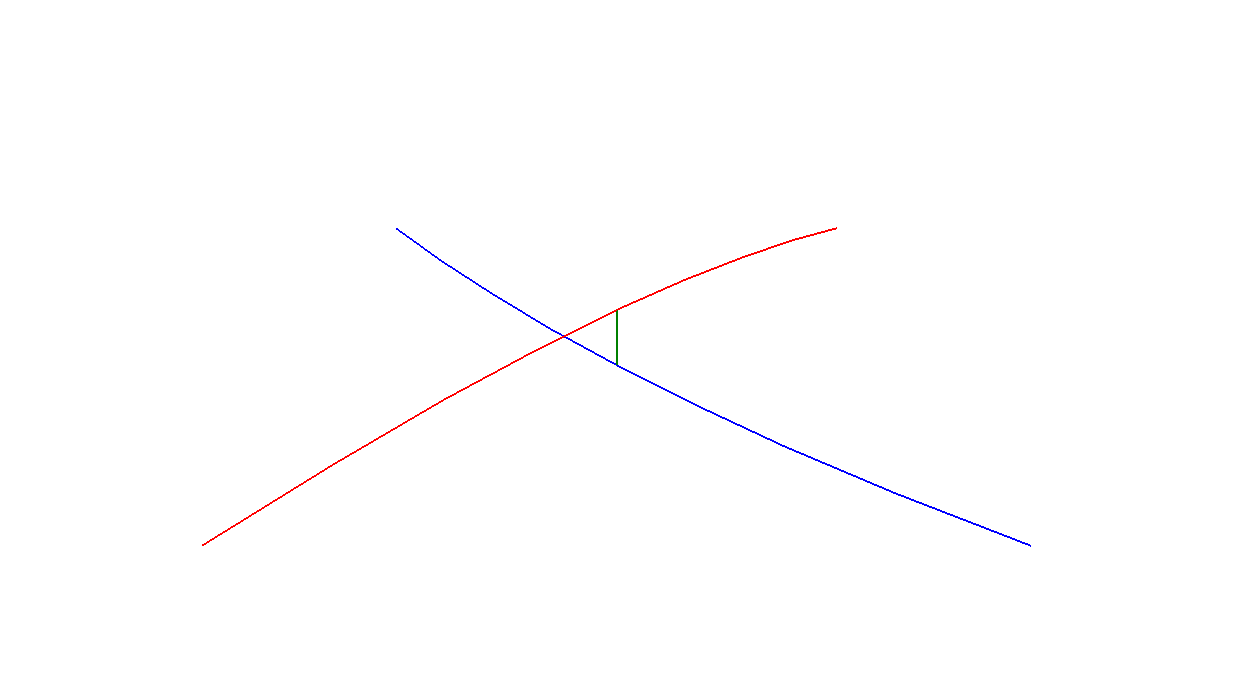
\includegraphics [width =\textwidth] {images/WireStentDemot2Step09}
	\begin{center}
	\vspace{-3ex}
	(c)
	\vspace{1ex}
	\end{center}
\end{minipage}
\hspace{0.3cm}	
   \end{latexonly}
   \begin{htmlonly}
     \htmladdimg{../images/WireStentDemot2Step04.png}
     \htmladdimg{../images/WireStentDemot2Step07.png}
     \htmladdimg{../images/WireStentDemot2Step09.png}
   \end{htmlonly}
	\caption {Creation of unit cell of crossing and connected struts (c) from a rescaled (a) and mirrored, skewed (b) bumped strut.} 
	\label{base}	
\end{figure}

\subsection{Extending the base module}

Subsequently, a mirrored copy of the base cell is generated. Both Formices are translated to their appropriate side by side position with the \code{translate()}-option and form the complete extended base module with 4 by 4 dimensions as depicted in Figure~\ref{fig:base}. Furthermore, both Formices are defined as an attribute of the \code{DoubleHelixStent} class by the \code{self}-statement, allowing their use after every \code{DoubleHelixStent} initialisation. Such further use is impossible with local variables, such as for example the \code{NE} and \code{SE} Formices.
%
\verbatiminput{scripts/WireStent5.py}

\begin{figure} [ht]
   \centering
   \begin{makeimage}
   \end{makeimage}
   \begin{latexonly}
	\hspace{0.1cm}
	\begin{minipage} [c] [] [c]{5.5cm} 
	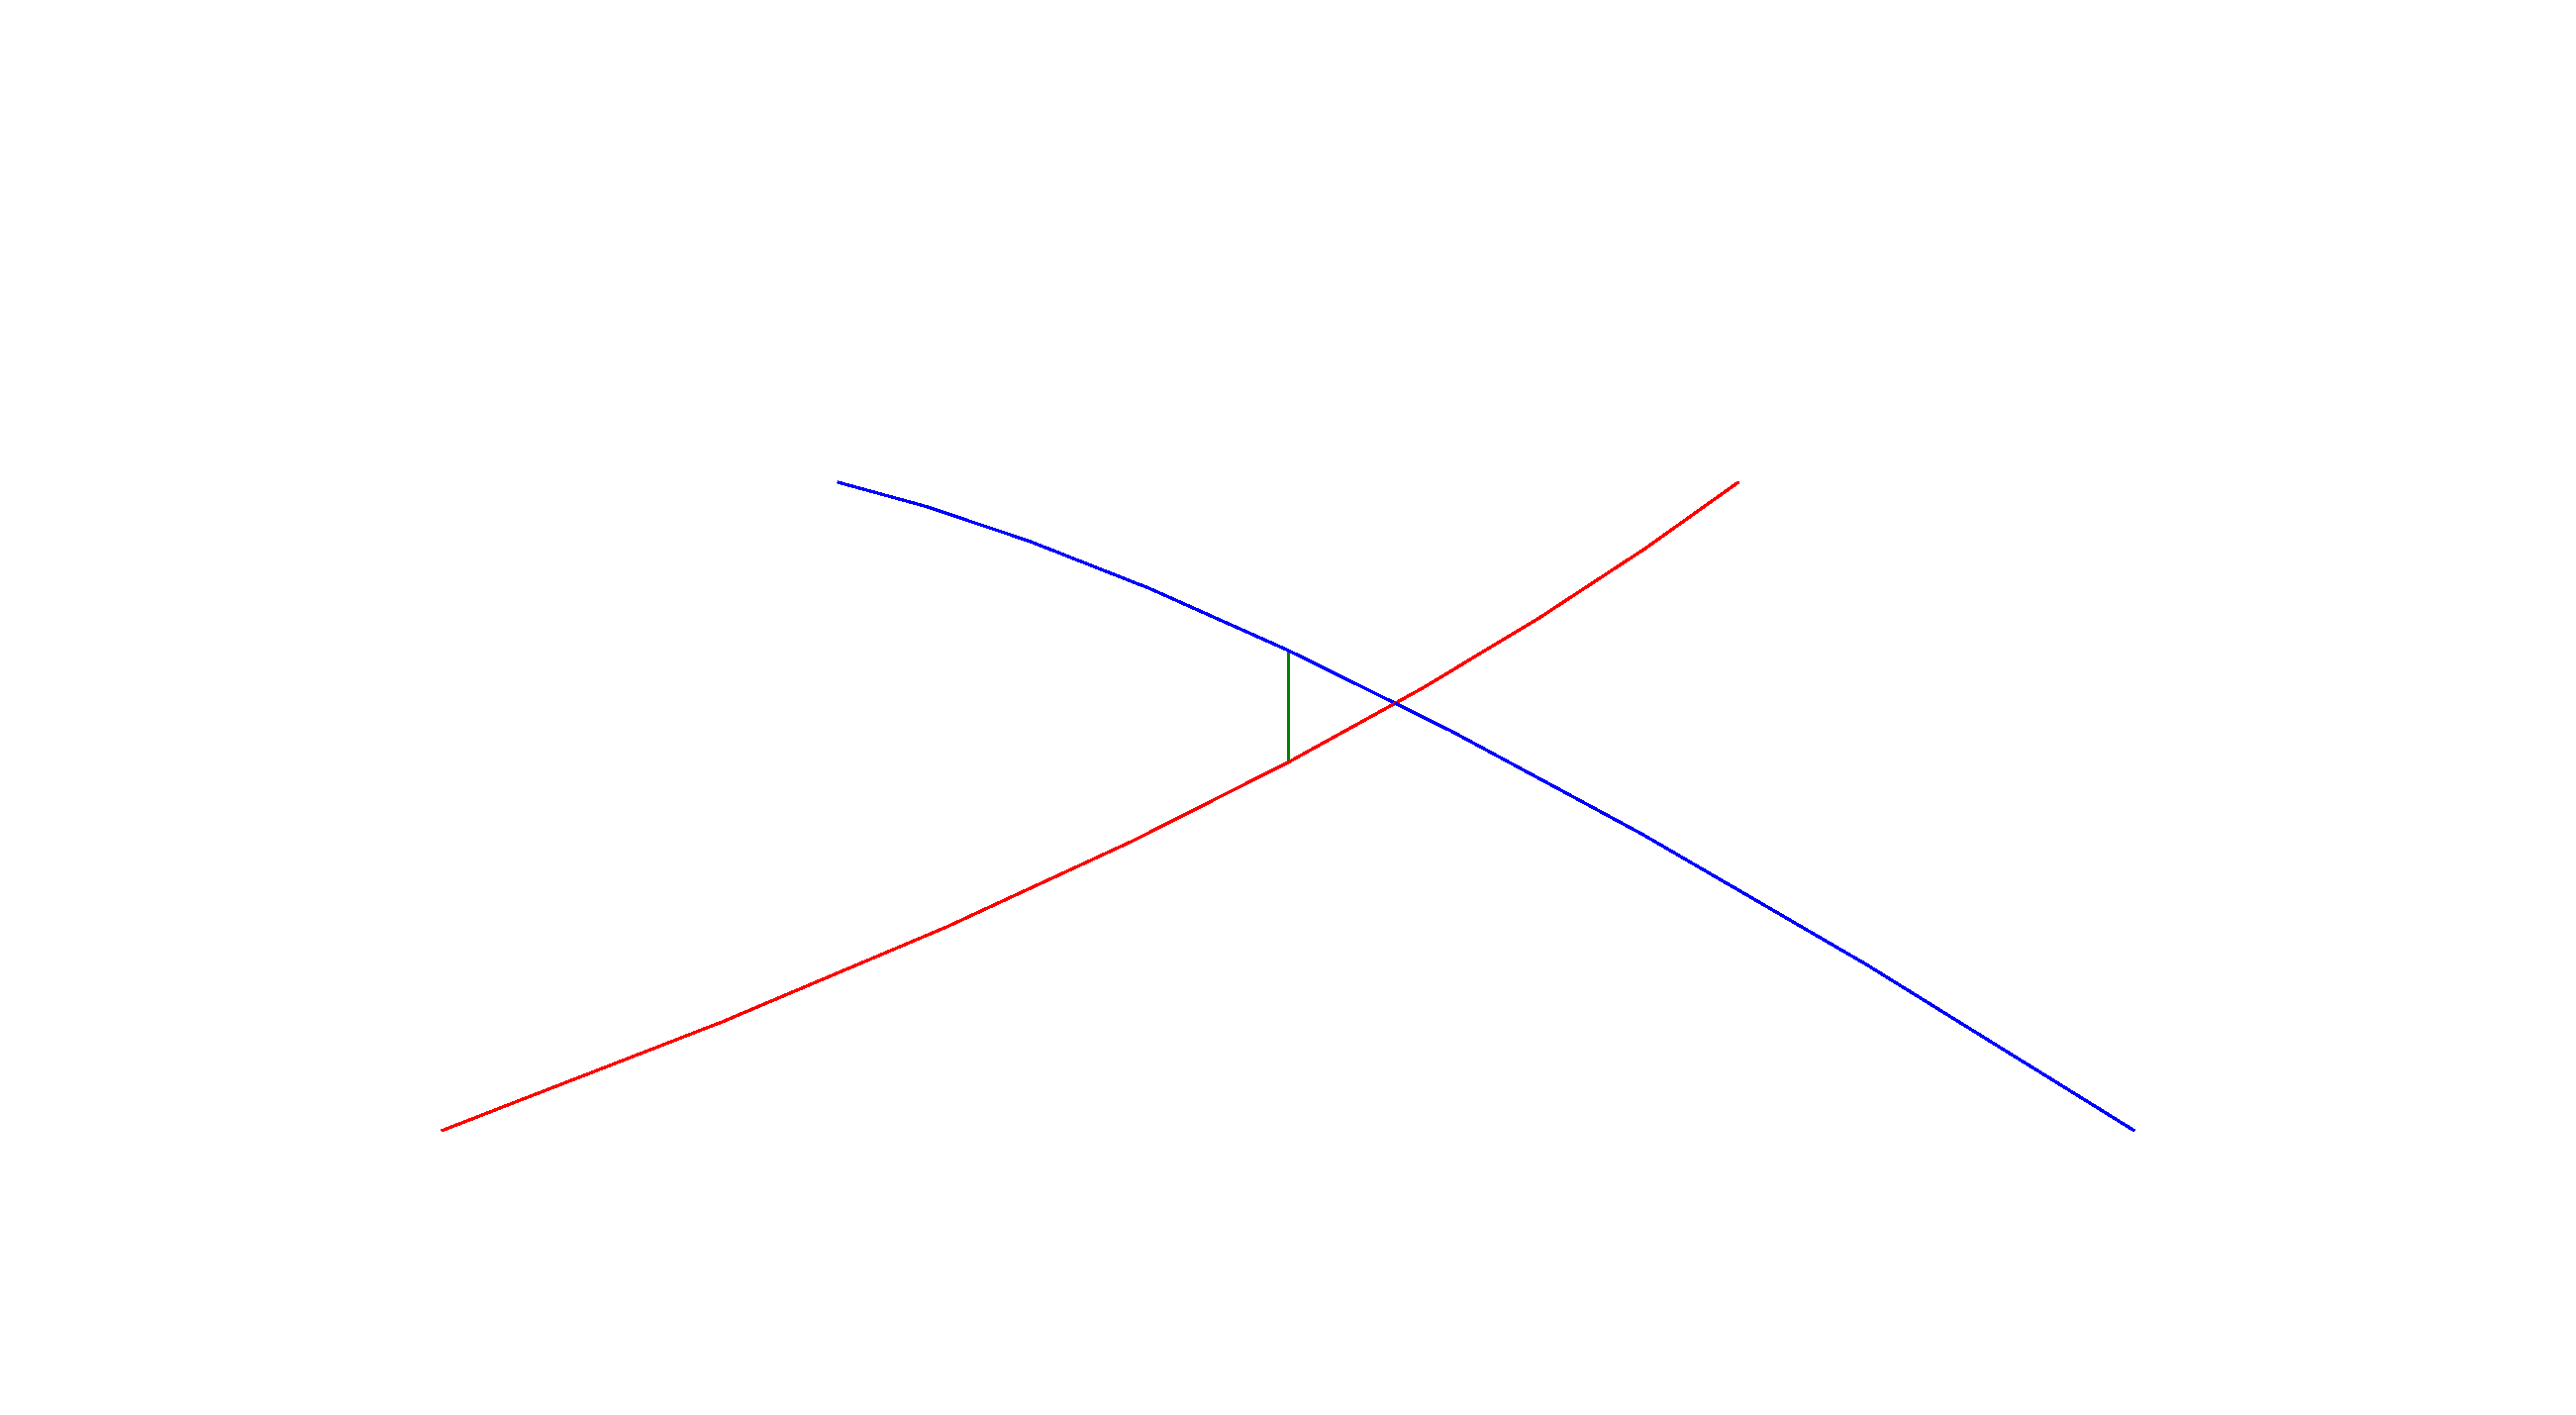
\includegraphics [width =\textwidth] {images/WireStentDemot2Step10}
	\begin{center}
	\vspace{-3ex}
	(a)
	\vspace{1ex}
	\end{center}
\end{minipage}
\hspace{0.3cm}
\begin{minipage} [c] [] [c] {5.5cm}
	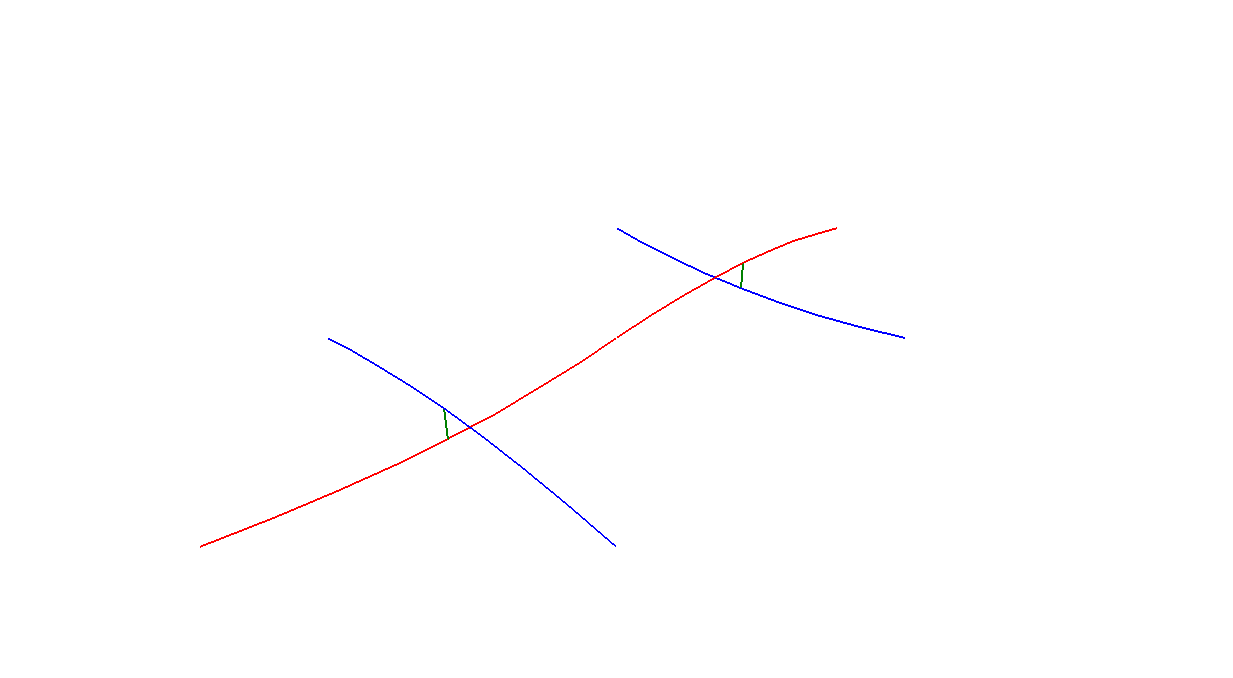
\includegraphics [width =\textwidth] {images/WireStentDemot2Step11}
	\begin{center}
	\vspace{-3ex}
	(b)
	\vspace{1ex}
	\end{center}
\end{minipage}
\hspace{0.3cm}
   \end{latexonly}
   \begin{htmlonly}
     \htmladdimg{../images/WireStentDemot2Step10.png}
     \htmladdimg{../images/WireStentDemot2Step11.png}
   \end{htmlonly} 
	\caption {Creation of the complete extended base module (b) from the original and mirrored (a) unit cell.} 
	\label{fig:base}
\end{figure}

\subsection{Full nearly planar pattern}

The fully nearly planar pattern is obtained by copying the base module in two directions and shown in Figure \ref{plane}. \code{replic2()} generates this pattern with $nx$ and $ny$ replications with steps $dx$ and $dy$ in respectively, the default X- and Y-direction.
%
\verbatiminput{scripts/WireStent6.py}

\begin{figure} [ht]
   \centering
   \begin{makeimage}
   \end{makeimage}
   \begin{latexonly}
	\hspace{0.1cm}
	\begin{minipage} [c] [] [c]{5.5cm} 
	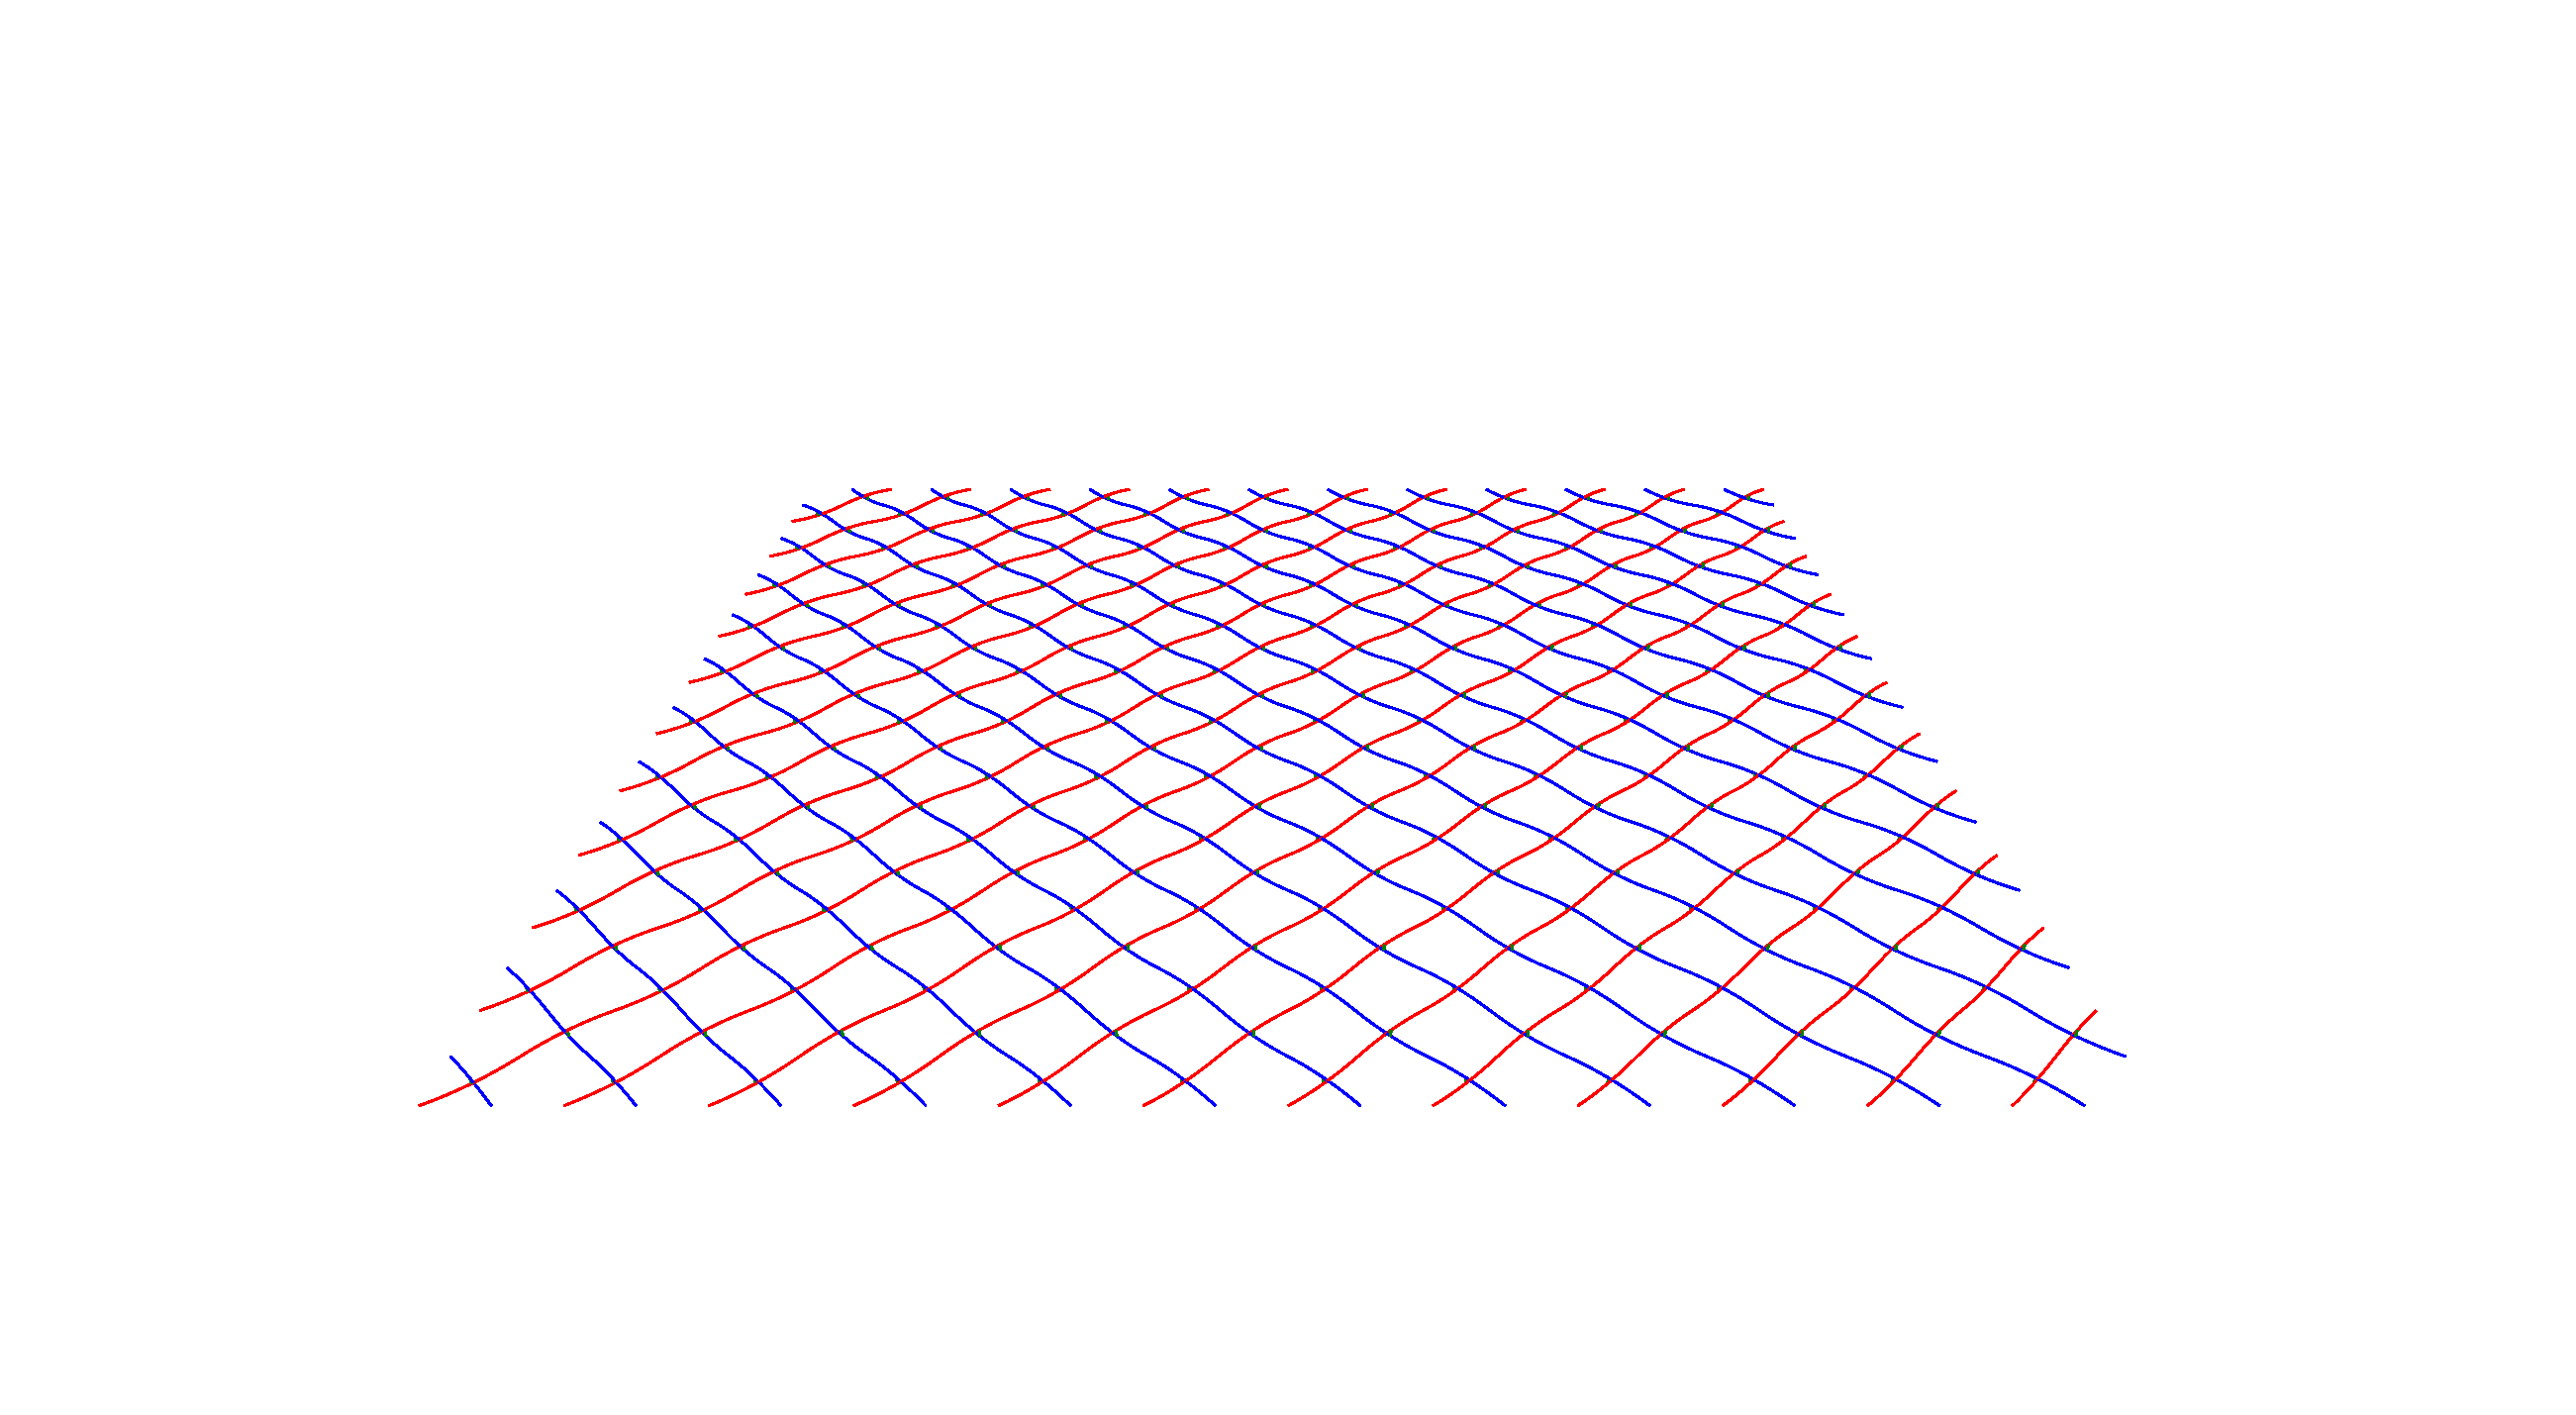
\includegraphics [width =\textwidth] {images/WireStentDemot2Step12}
	\begin{center}
	\vspace{-3ex}
	%(a)
	\vspace{1ex}
	\end{center}
\end{minipage}
\hspace{0.3cm}
\begin{minipage} [c] [] [c] {5.5cm}
	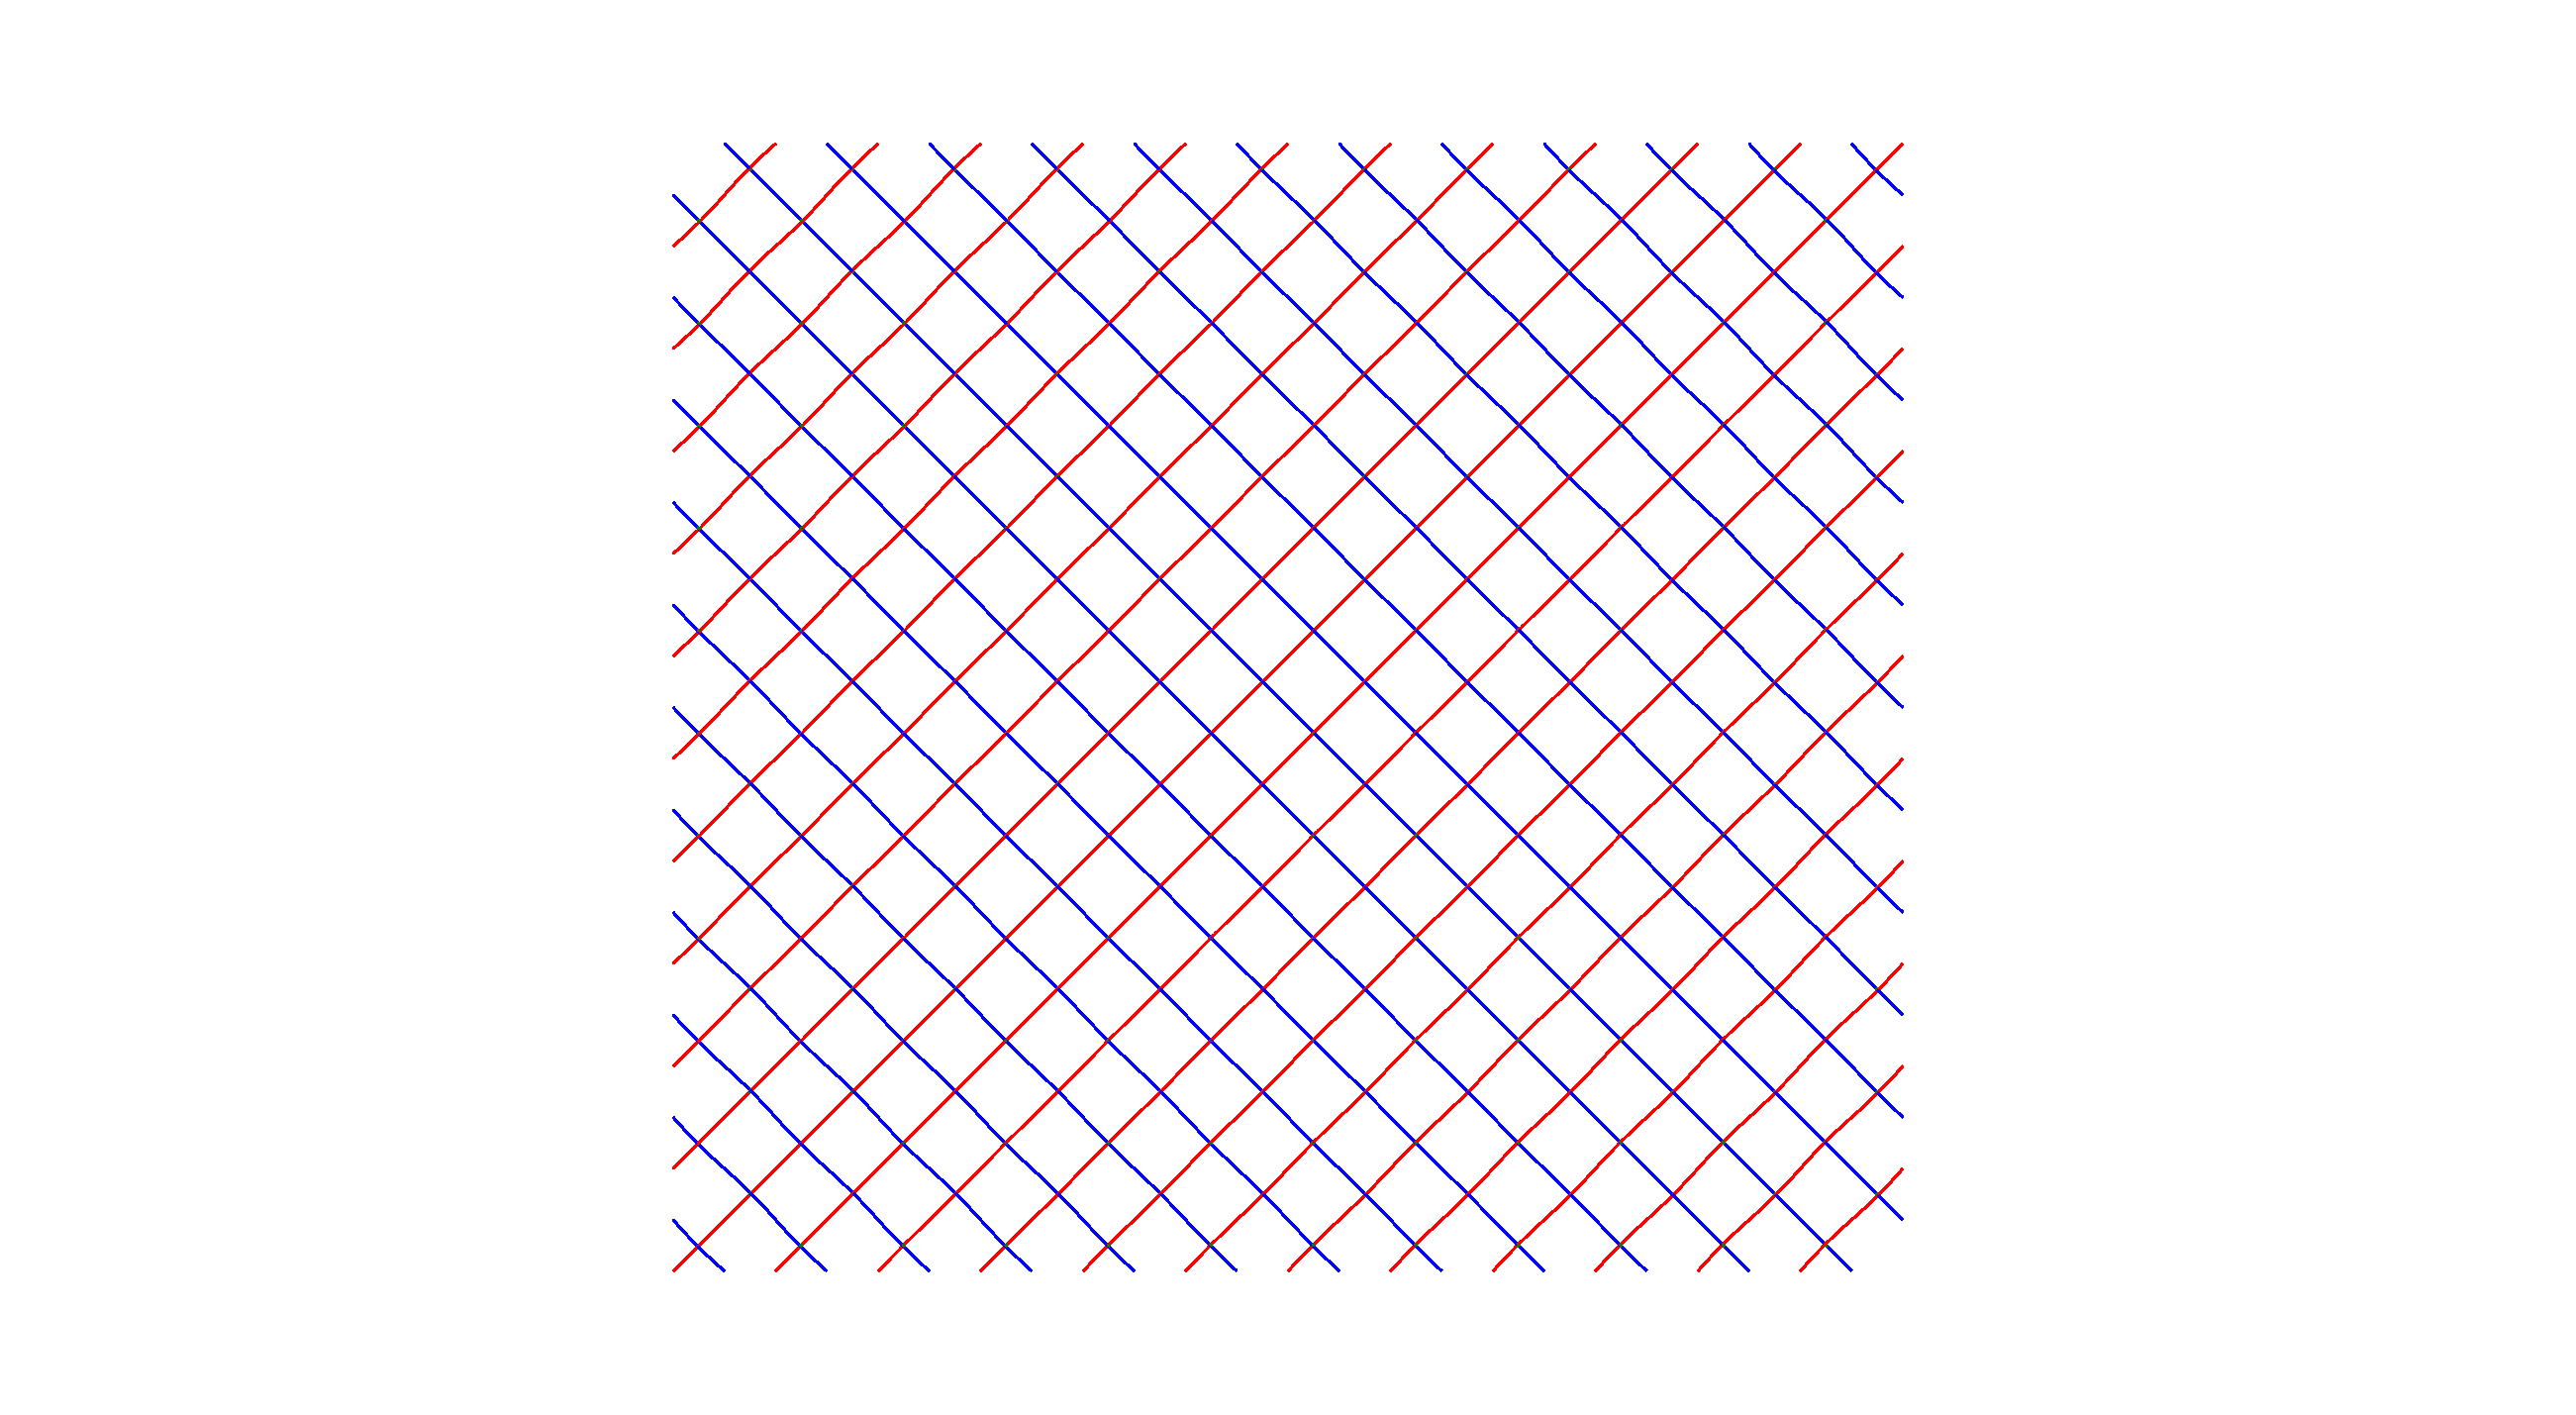
\includegraphics [width =\textwidth] {images/WireStentDemot2Step13}
	\begin{center}
	\vspace{-3ex}
	%(b)
	\vspace{1ex}
	\end{center}
\end{minipage}
\hspace{0.3cm}
   \end{latexonly}
   \begin{htmlonly}
     \htmladdimg{../images/WireStentDemot2Step12.png}
     \htmladdimg{../images/WireStentDemot2Step13.png}
   \end{htmlonly} 
	\caption {Creation of the fully nearly planar pattern.} 
	\label{plane}	
\end{figure}

\subsection{Cylindrical stent structure}

Finally the full pattern is translated over the stent radius $r$ in Z-direction and transformed to the cylindrical stent structure by a coordinate transformation with the Z-coordinates as distance $r$, the X-coordinates as angle $\theta$ and the Y-coordinates as height $z$. The \code{scale()}-operator rescales the stent structure to the correct circumference and length. The resulting stent geometry is depicted in Figure \ref{stent}.
%
\verbatiminput{scripts/WireStent7.py}

\begin{figure} [ht]
   \centering
   \begin{makeimage}
   \end{makeimage}
   \begin{latexonly}
	\hspace{0.1cm}
	\begin{minipage} [c] [] [c]{5.5cm} 
	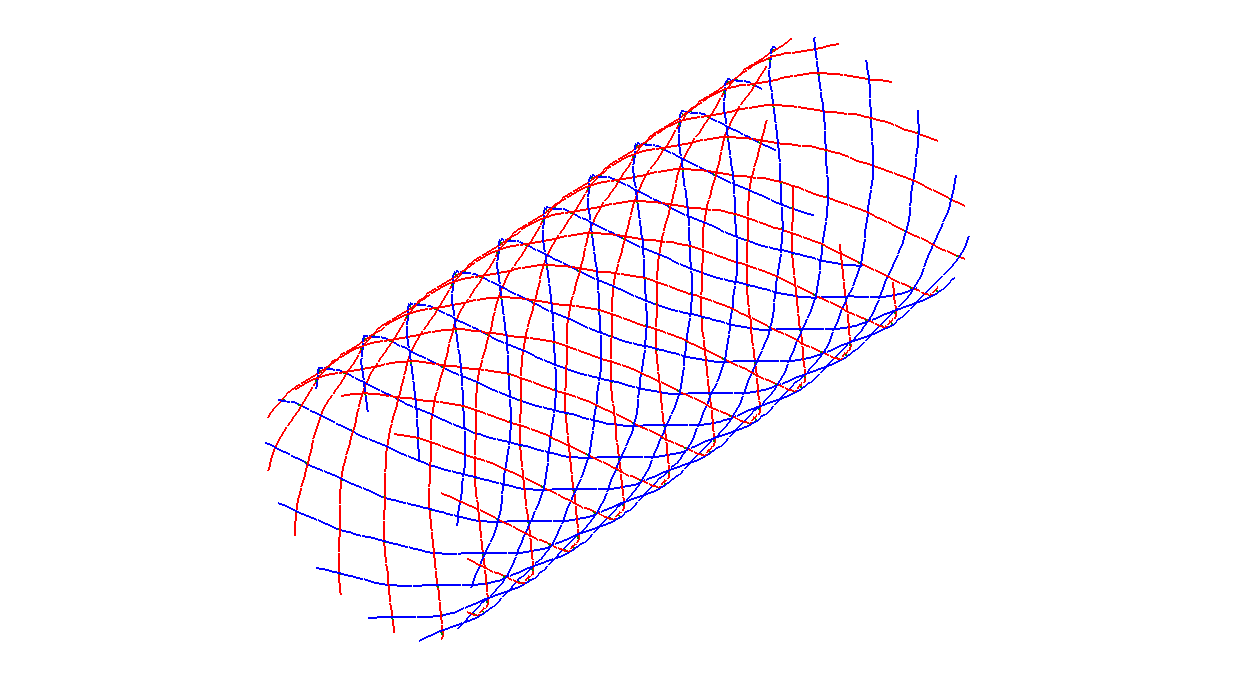
\includegraphics [width =\textwidth] {images/WireStentDemot2Step16}
	\begin{center}
	\vspace{-3ex}
	(a)
	\vspace{1ex}
	\end{center}
\end{minipage}
\hspace{0.3cm}
\begin{minipage} [c] [] [c] {5.5cm}
	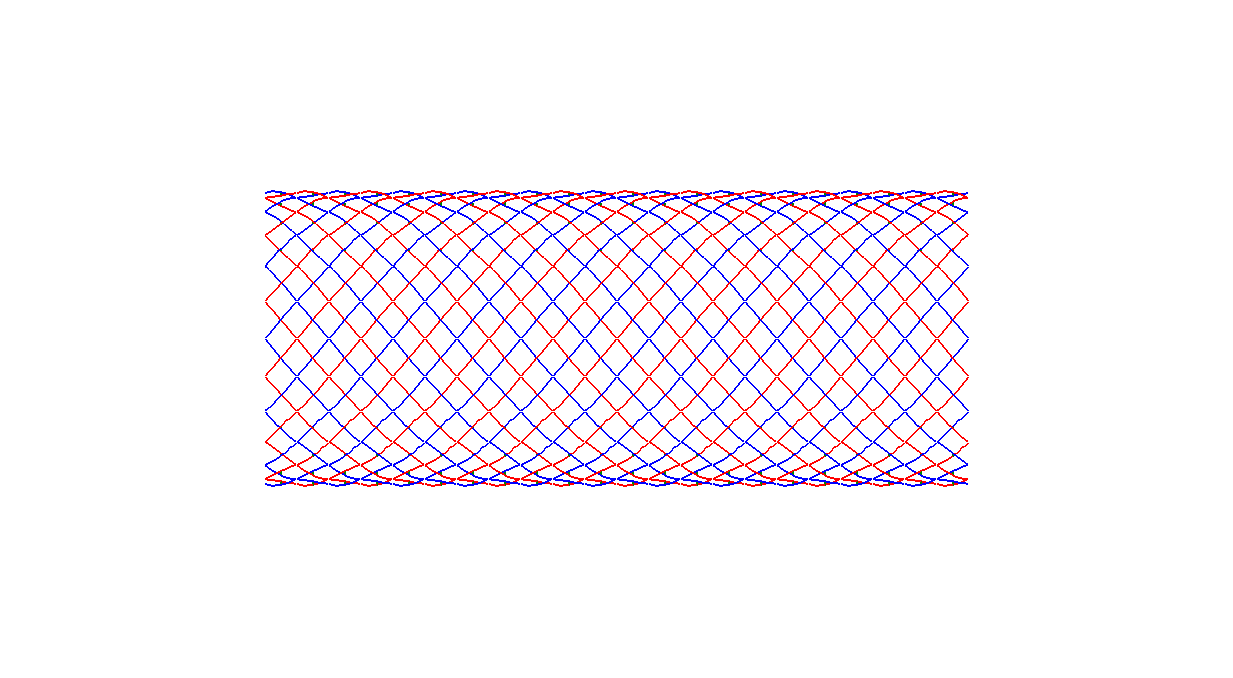
\includegraphics [width =\textwidth] {images/WireStentDemot2Step15}
	\begin{center}
	\vspace{-3ex}
	(b)
	\vspace{1ex}
	\end{center}
\end{minipage}
\hspace{0.3cm}
   \end{latexonly}
   \begin{htmlonly}
     \htmladdimg{../images/WireStentDemot2Step16.png}
     \htmladdimg{../images/WireStentDemot2Step15.png}
   \end{htmlonly}
	\caption {Creation of the cylindrical stent structure ((a) iso and (b) right view).} 
	\label{stent}	
\end{figure}

In addition to the stent initialization, the \code{DoubleHelixStent} class script contains a function \code{all()} representing the complete stent Formex. Consequently, the \code{DoubleHelixStent} class has four attributes: the Formices \code{cell1}, \code{cell2} and \code{all}; and the number $ny$.
%
\verbatiminput{scripts/WireStent8.py}

%
\subsection{Parametric stent geometry}
%
An inherent feature of script-based modeling is the possibility of easily generating lots of variations on the original geometry. This is a huge advantage for parametric analyses and illustrated in Figure \ref{param}: these wire stents are all created with the same script, but with other values of the parameters $De$, $nx$ and $\beta$. As the script for building the wire stent geometry is defined as a the \code{DoubleHelixStent} class in the (\file{WireStent.py}) script, it can easily be imported for e.g. this purpose.

\begin{figure} [ht]
   \centering
   \begin{makeimage}
   \end{makeimage}
   \begin{latexonly}
	\hspace{0.1cm}
	\begin{minipage} [c] [] [c]{5.5cm} 
	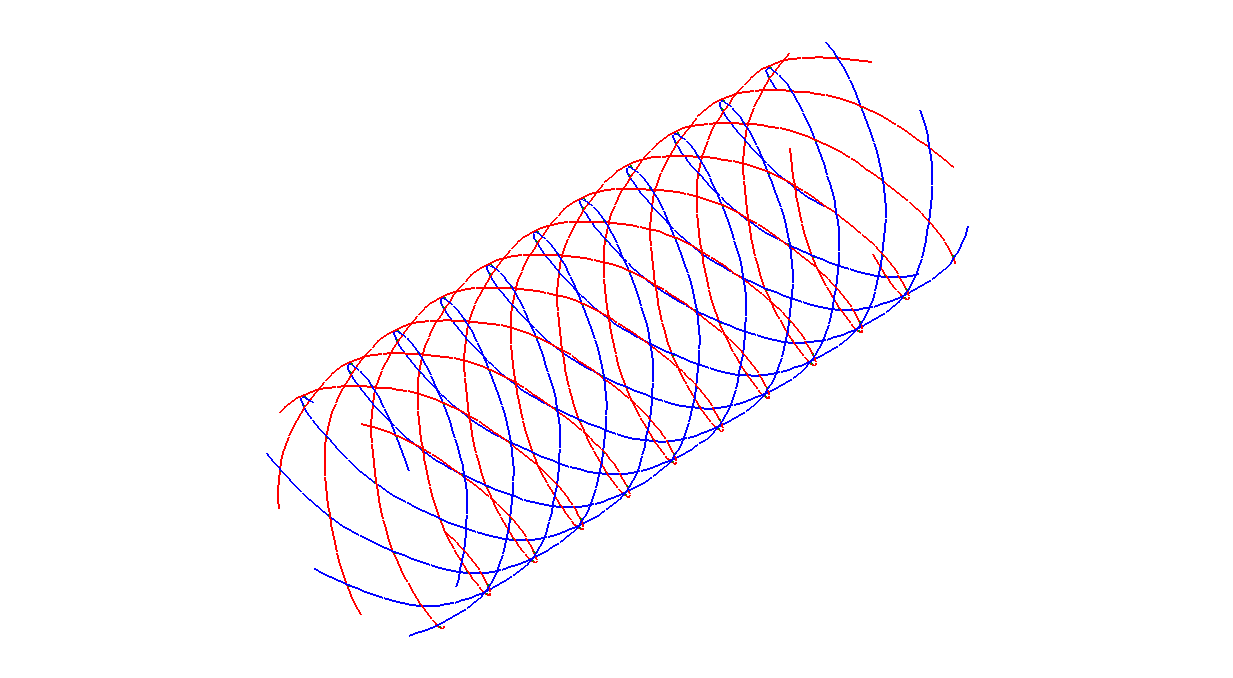
\includegraphics [width =\textwidth] {images/WireStentD16L40d22n6b25}
	\begin{center}
	\vspace{-3ex}
	\code{DHS}(16,40,0.22,6,25)
	\vspace{1ex}
	\end{center}
\end{minipage}
\hspace{0.3cm}
\begin{minipage} [c] [] [c] {5.5cm}
	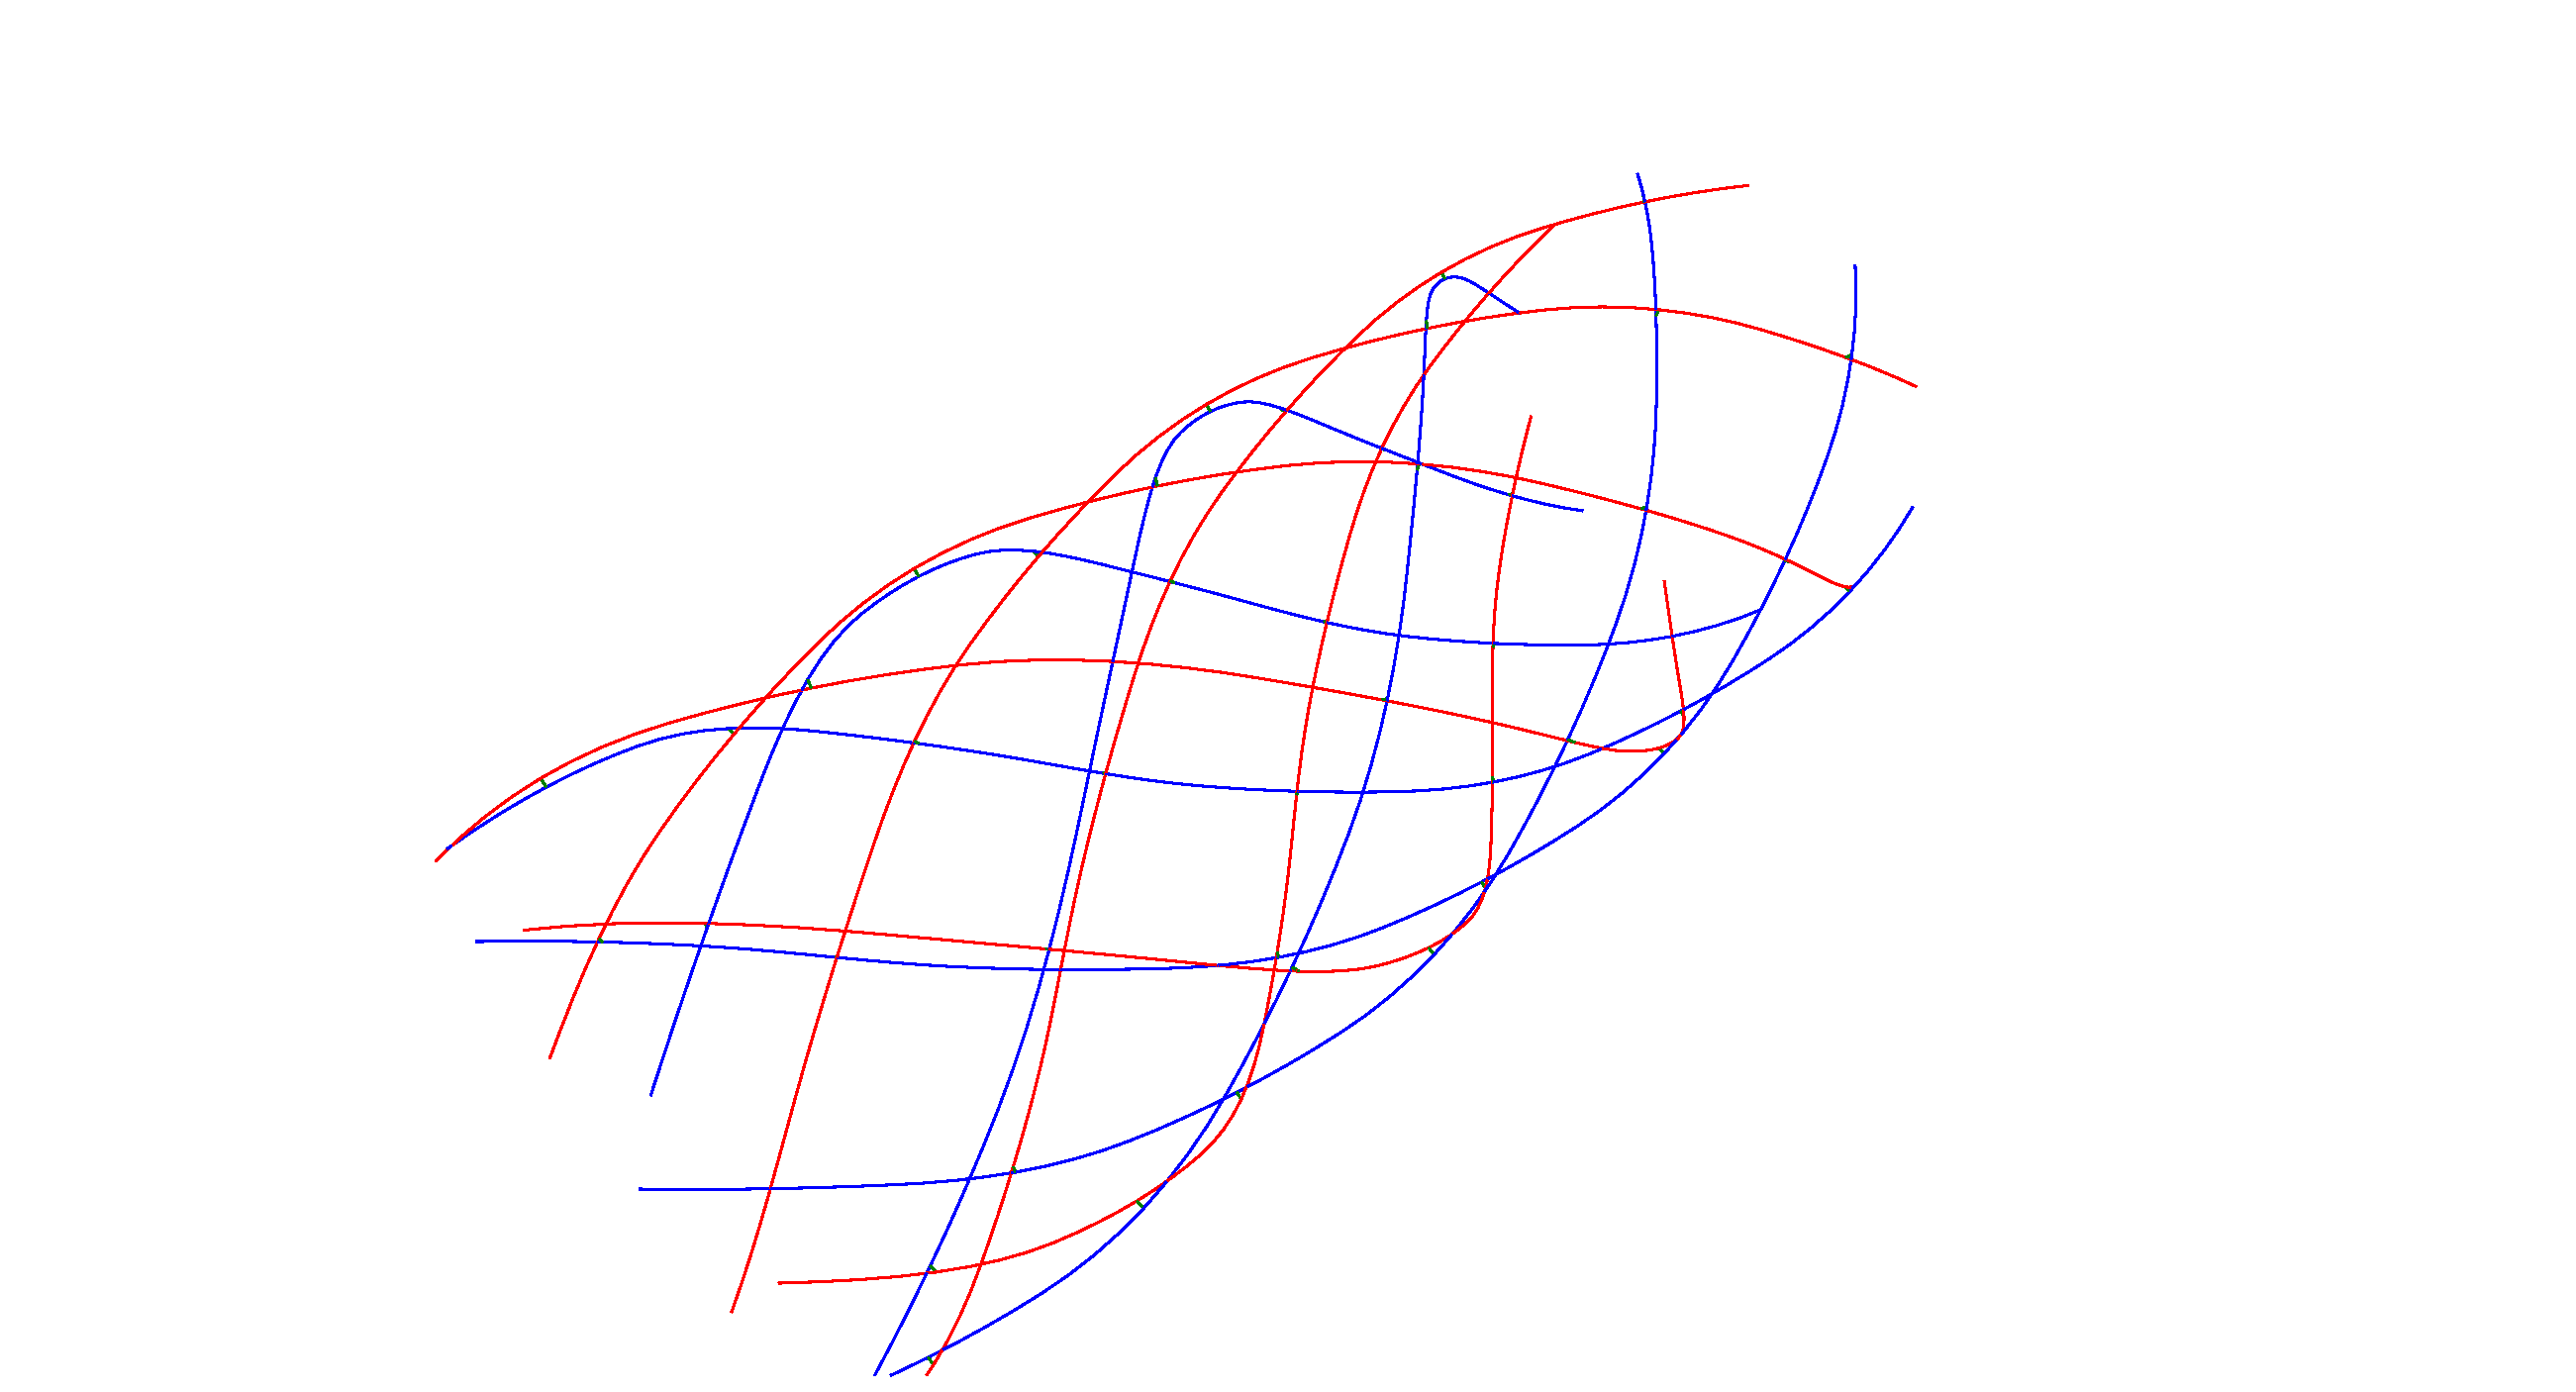
\includegraphics [width =\textwidth] {images/WireStentD16L40d22n6b50}
	\begin{center}
	\vspace{-3ex}
	\code{DHS}(16,40,0.22,6,50)
	\vspace{1ex}
	\end{center}
\end{minipage}
\hspace{0.3cm}
\hspace{0.1cm}
	\begin{minipage} [c] [] [c]{5.5cm} 
	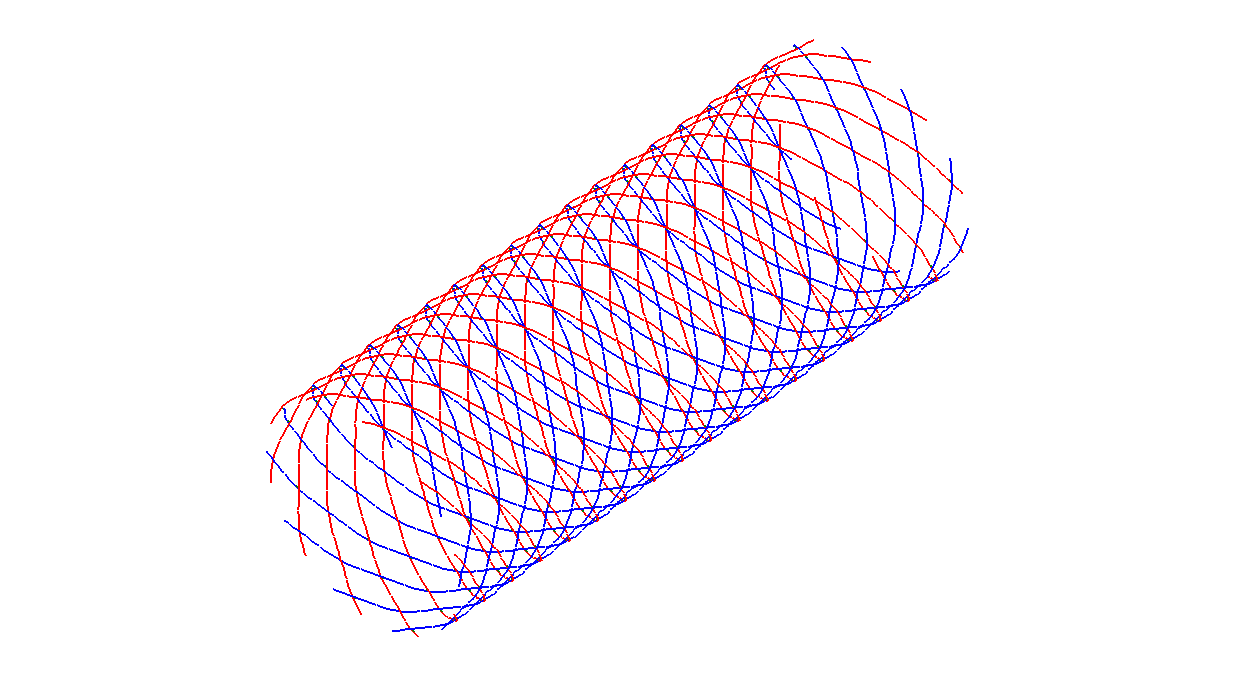
\includegraphics [width =\textwidth] {images/WireStentD16L40d22n10b25}
	\begin{center}
	\vspace{-3ex}
	\code{DHS}(16,40,0.22,10,25)
	\vspace{1ex}
	\end{center}
\end{minipage}
\hspace{0.3cm}
\begin{minipage} [c] [] [c] {5.5cm}
	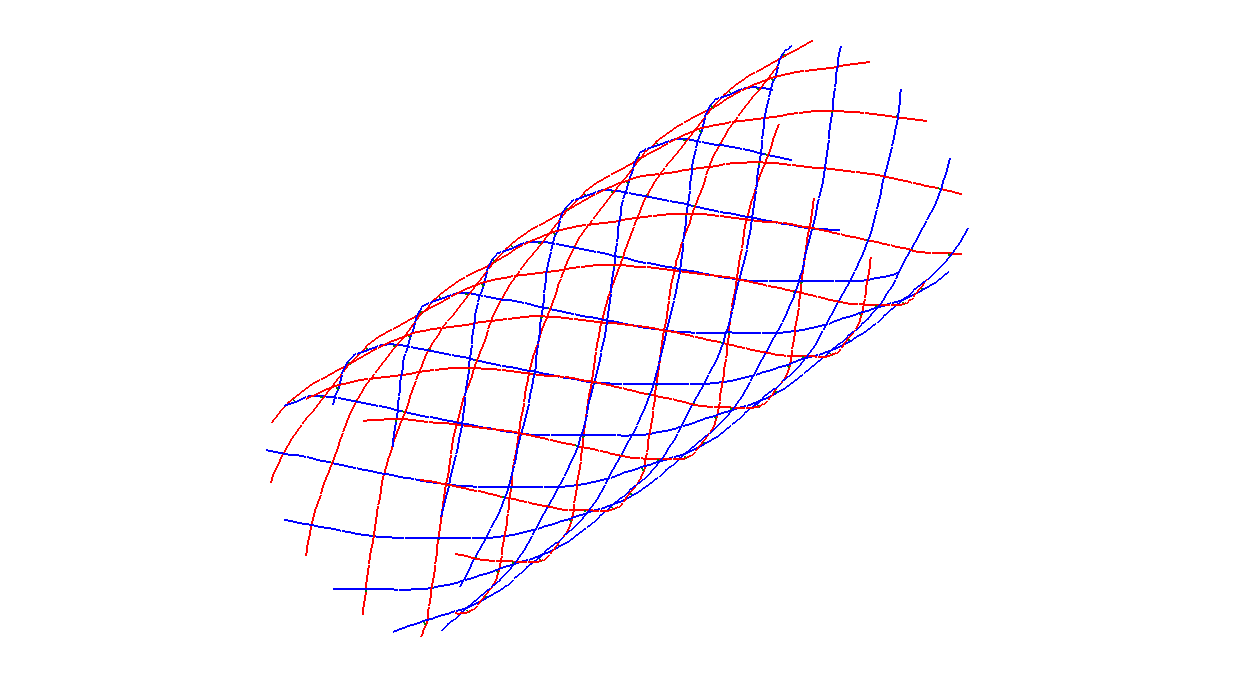
\includegraphics [width =\textwidth] {images/WireStentD16L40d22n10b50}
	\begin{center}
	\vspace{-3ex}
	\code{DHS}(16,40,0.22,10,50)
	\vspace{1ex}
	\end{center}
\end{minipage}
\hspace{0.3cm}
\hspace{0.1cm}
	\begin{minipage} [c] [] [c]{5.5cm} 
	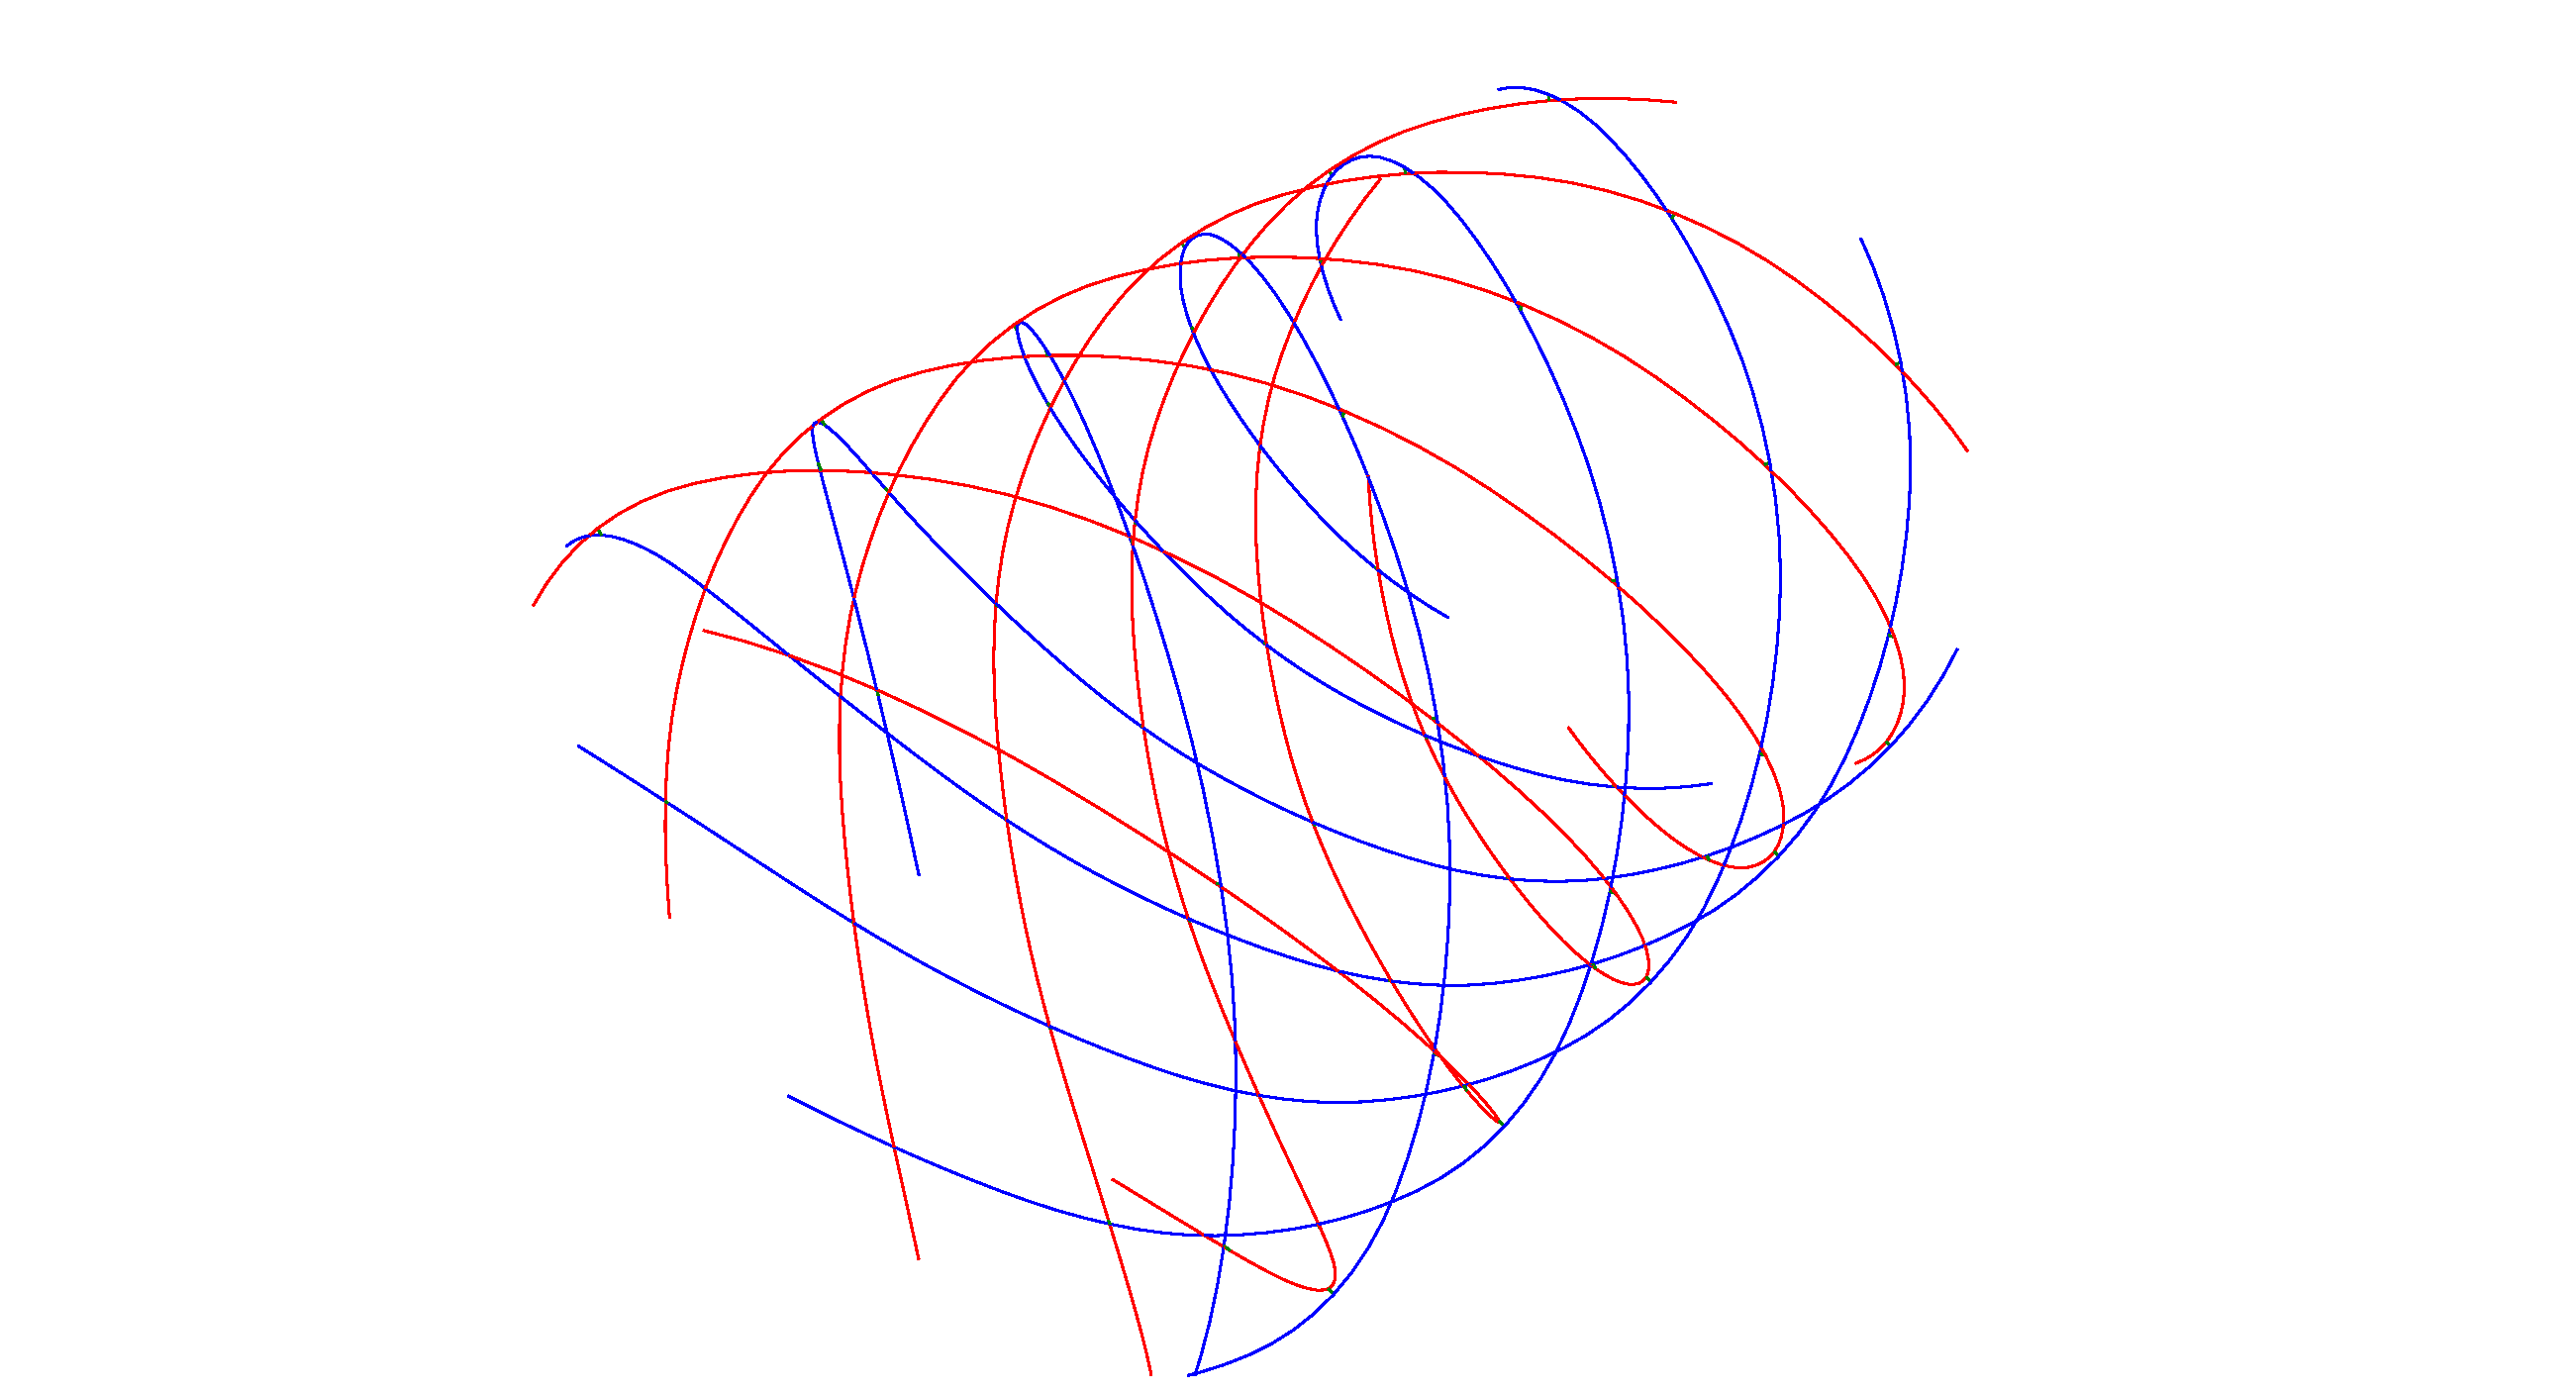
\includegraphics [width =\textwidth] {images/WireStentD32L40d22n6b25}
	\begin{center}
	\vspace{-3ex}
	\code{DHS}(32,40,0.22,6,25)
	\vspace{1ex}
	\end{center}
\end{minipage}
\hspace{0.3cm}
\begin{minipage} [c] [] [c] {5.5cm}
	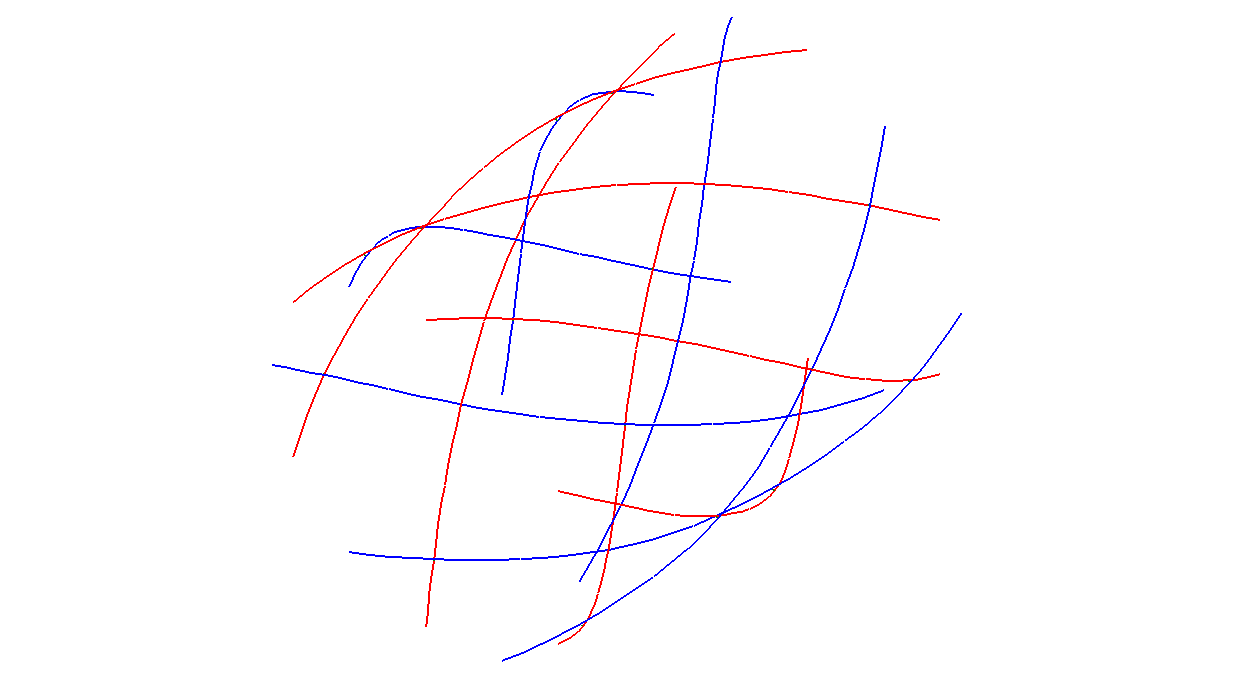
\includegraphics [width =\textwidth] {images/WireStentD32L40d22n6b50}
	\begin{center}
	\vspace{-3ex}
	\code{DHS}(32,40,0.22,6,50)
	\vspace{1ex}
	\end{center}
\end{minipage}
\hspace{0.3cm}
\hspace{0.1cm}
	\begin{minipage} [c] [] [c]{5.5cm} 
	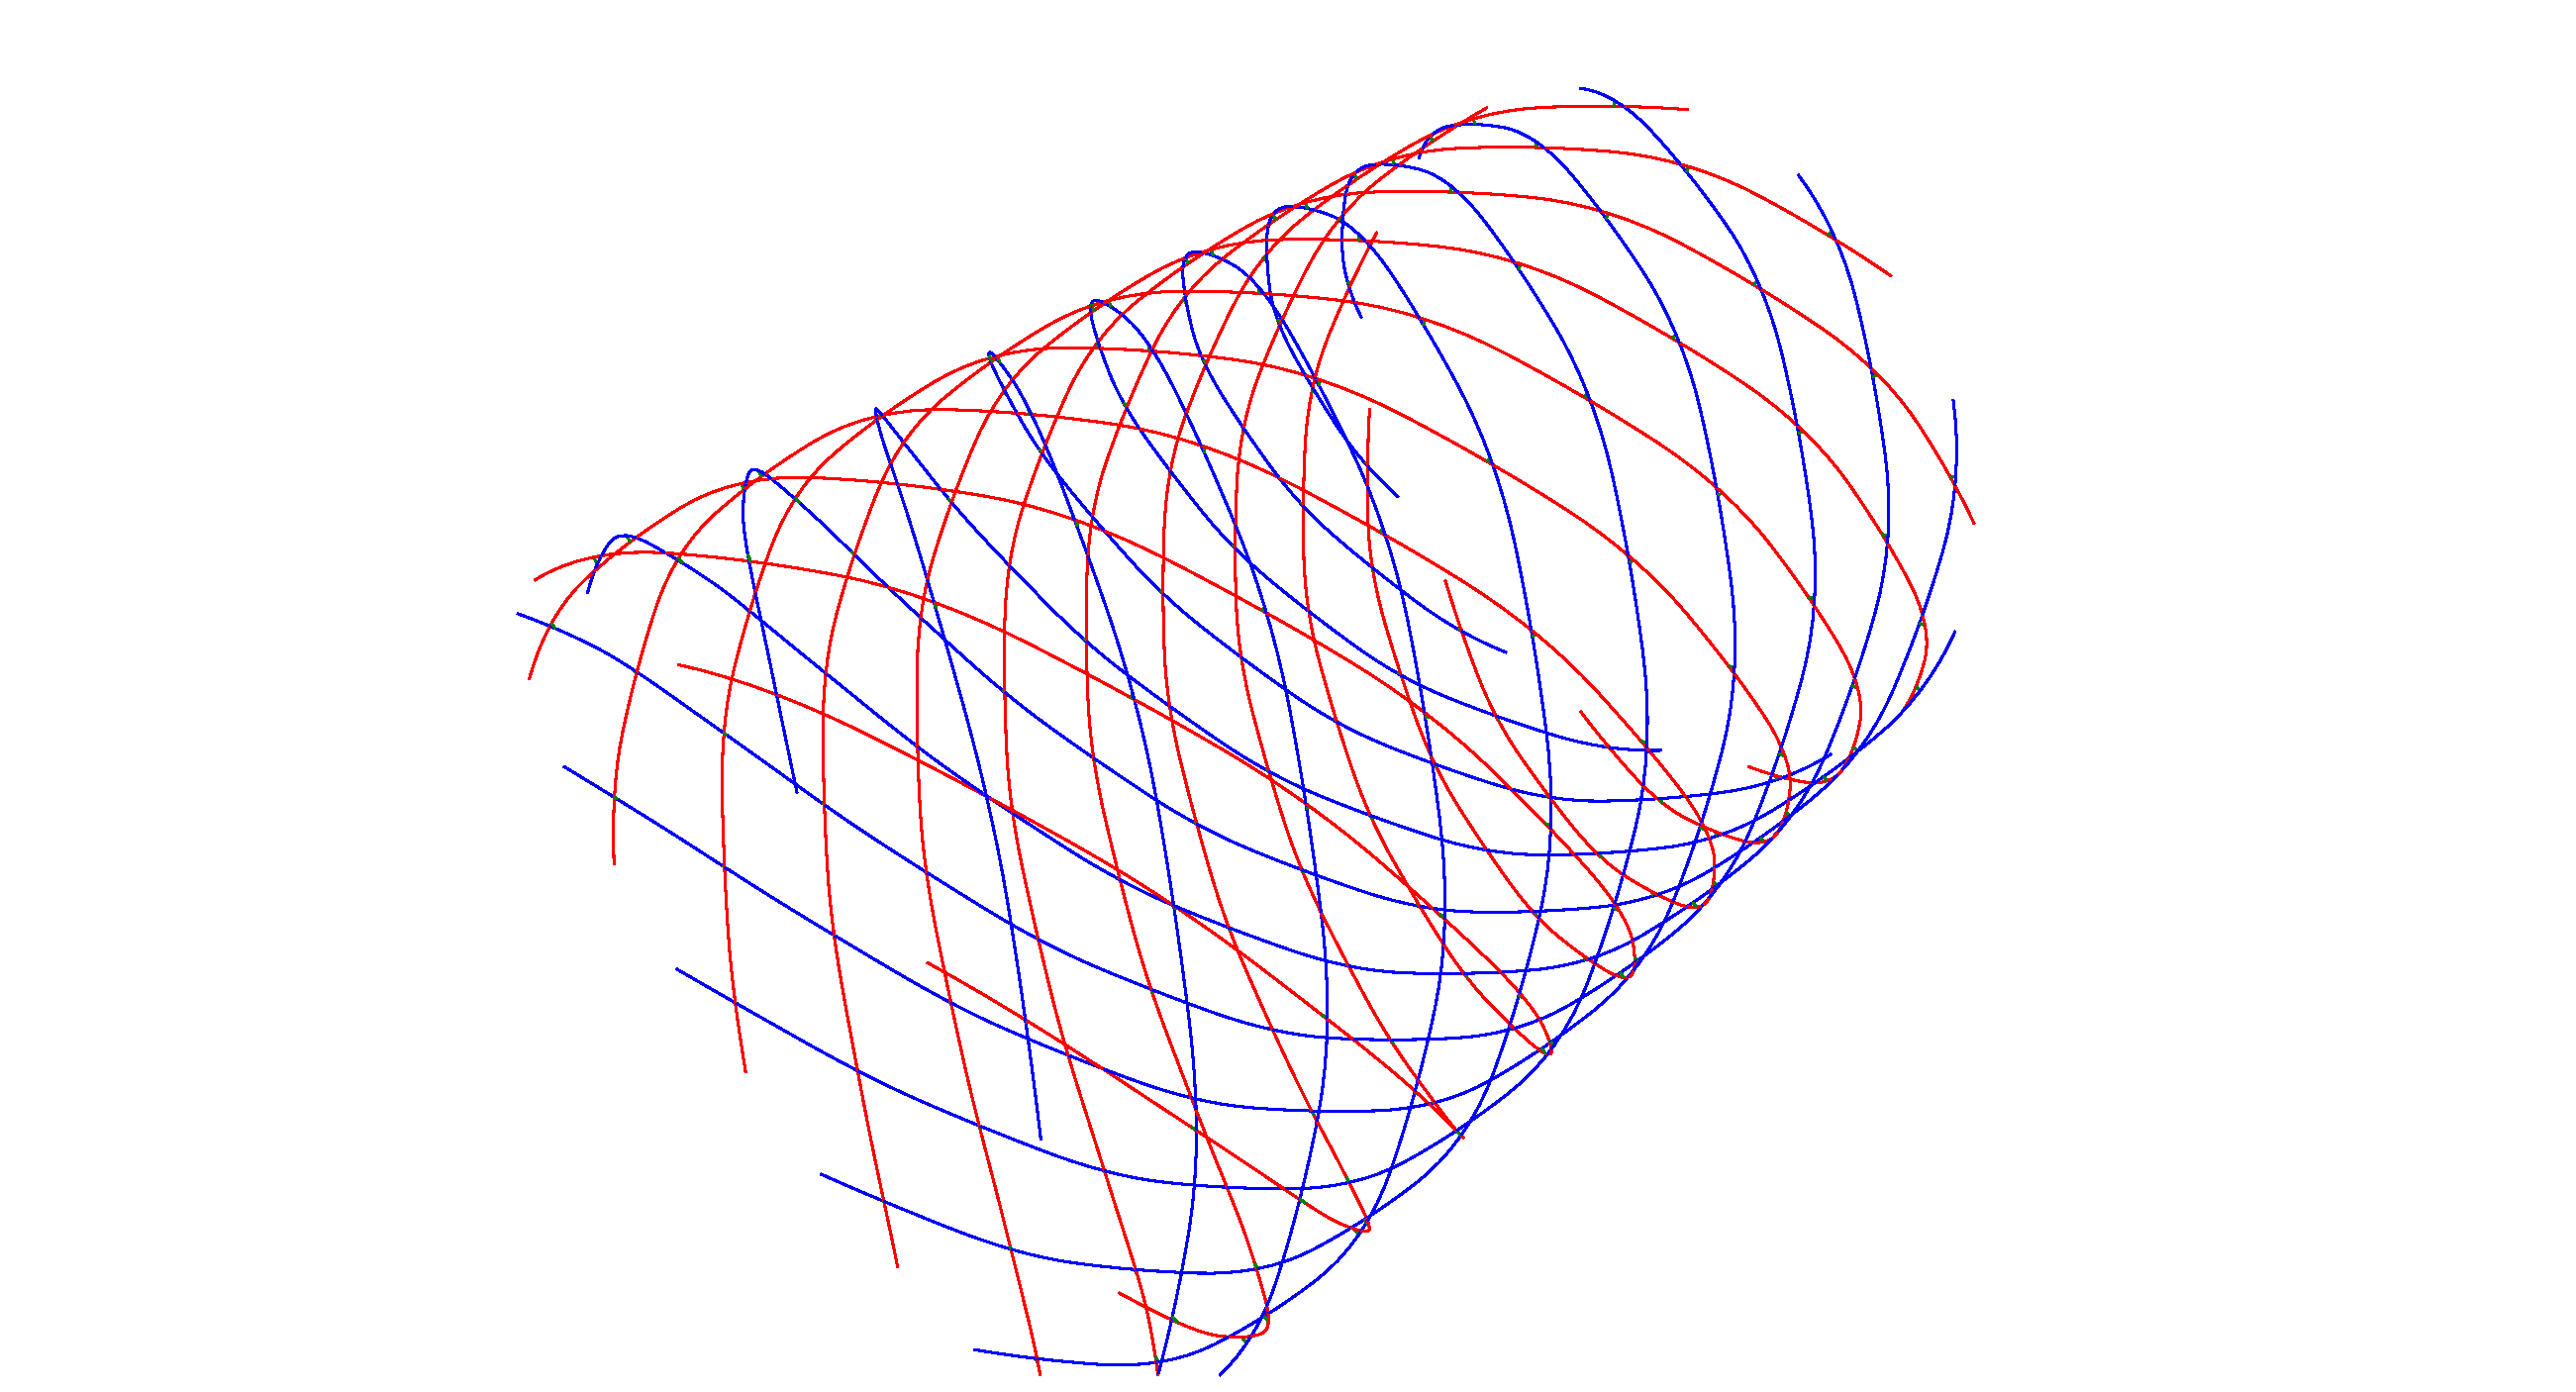
\includegraphics [width =\textwidth] {images/WireStentD32L40d22n10b25}
	\begin{center}
	\vspace{-3ex}
	\code{DHS}(32,40,0.22,10,25)
	\vspace{1ex}
	\end{center}
\end{minipage}
\hspace{0.3cm}
\begin{minipage} [c] [] [c] {5.5cm}
	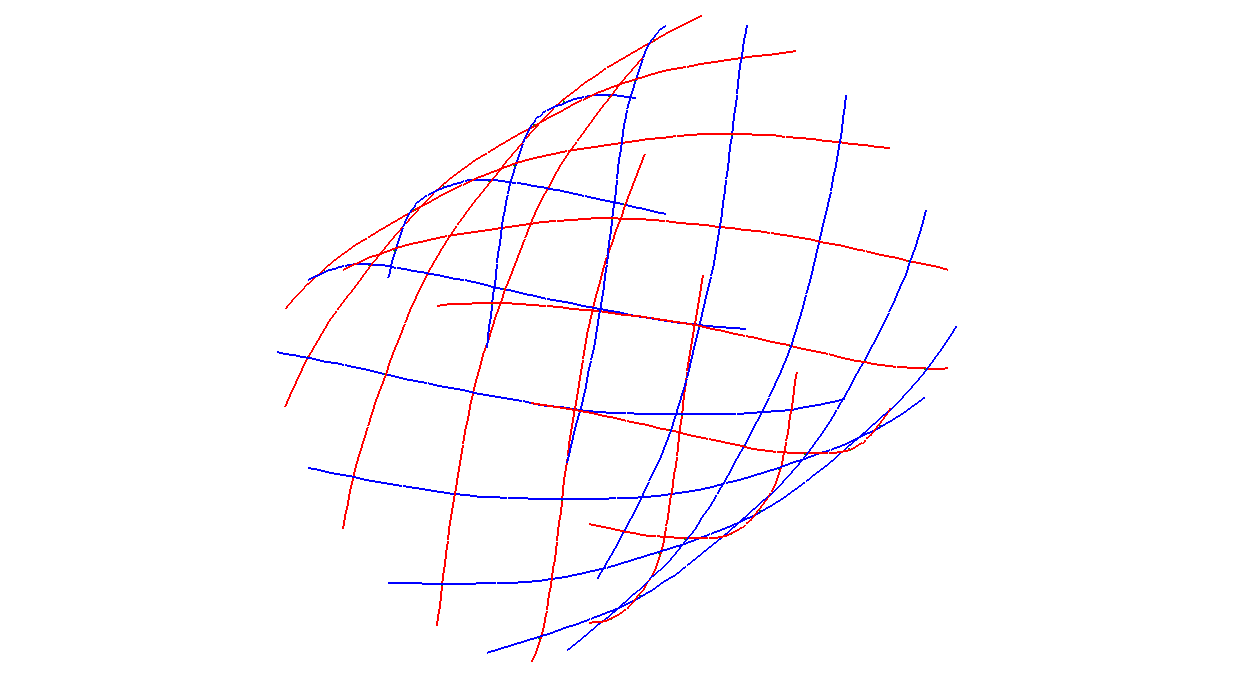
\includegraphics [width =\textwidth] {images/WireStentD32L40d22n10b50}
	\begin{center}
	\vspace{-3ex}
	\code{DHS}(32,40,0.22,10,50)
	\vspace{1ex}
	\end{center}
\end{minipage}
\hspace{0.3cm}
   \end{latexonly}
   \begin{htmlonly}
     \htmladdimg{../images/WireStentD16L40d22n6b25.png}
     \htmladdimg{../images/WireStentD16L40d22n6b50.png}
     \htmladdimg{../images/WireStentD16L40d22n10b25.png}
     \htmladdimg{../images/WireStentD16L40d22n10b50.png}
     \htmladdimg{../images/WireStentD32L40d22n6b25.png}
     \htmladdimg{../images/WireStentD32L40d22n6b50.png}
     \htmladdimg{../images/WireStentD32L40d22n10b25.png}
     \htmladdimg{../images/WireStentD32L40d22n10b50.png}
   \end{htmlonly} 
	\caption {Variations on the wire stent geometry using the DoubleHelixStent($De,L,d,nx,\beta$) (DHS() class.} 
	\label{param} 	
\end{figure}

\verbatiminput{scripts/WireStentParametricExample.py}

Obviously, generating such parametric wire stent geometries with classical CAD methodologies is feasible, though probably (very) time consuming. However, as \pyf provides a multitude of features (such as parametric modeling, finite element pre- and postprocessing, optimization strategies, etcetera) in one sinlge consistent environment, it appearss to be the obvious way to go when studying the mechanical behavior of braided wire stents.

\newpage

\section{Operating on surface meshes}
\label{sec:operating-surf-mesh}

Besides being used for creating geometries, \pyf also offers interesting possibilities for executing specialized operations on surface meshes, usually STL type triangulated meshes originating from medical scan (CT) images. Some of the algorithms developed were included in \pyf.

\subsection{Unroll stent}
\label{sec:unroll-stent}

A stent is a medical device used to reopen narrowed arteries. The vast majority of stents are balloon-expandable, which means that the metal structure is deployed by inflating a balloon, located inside the stent. Figure~\ref{fig:cypher-stent} shows an example of such a stent prior to expansion (balloon not shown). The 3D surface is obtained by micro CT and consists of triangles.

\begin{figure}[ht]
  \centering
  \begin{makeimage}
  \end{makeimage}
  \begin{latexonly}
    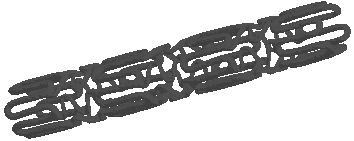
\includegraphics[width=8cm]{images/cypher-stent}
  \end{latexonly}
  \begin{htmlonly}
    \htmladdimg{../images/cypher-stent.png}
  \end{htmlonly}  
  \caption{Triangulated mesh of a stent}
  \label{fig:cypher-stent}
\end{figure}

The structure of such a device can be quite complex and difficult to analyse. The same functions \pyf offers for creating geometries can also be employed to investigate triangulated meshes. A simple unroll operation of the stent gives a much better overview of the complete geometrical structure and allows easier analysis (see figure~\ref{fig:cypher-stent-unroll}).
 
\code{F = F.toCylindrical().scale([1.,2*radius*pi/360,1.])}

\begin{figure}[ht]
  \centering
  \begin{makeimage}
  \end{makeimage}
  \begin{latexonly}
    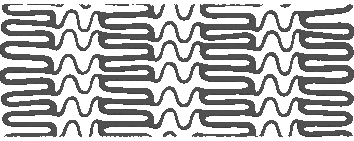
\includegraphics[width=8cm]{images/cypher-stent-unroll}
  \end{latexonly}
  \begin{htmlonly}
    \htmladdimg{../images/cypher-stent-unroll.png}
  \end{htmlonly}  
  \caption{Result of unroll operation}
  \label{fig:cypher-stent-unroll}
\end{figure}

This unrolled geometry can then be used for further investigations. An important property of such a stent is the circumference of a single stent cell. The \code{clip()} method can be used to isolate a single stent cell. In order to obtain a line describing the stent cell, the function \code{intersectionLinesWithPlane()} has been used. The result can be seen in figure~\ref{fig:stent-cell}.

\begin{figure}[ht]
  \centering
  \begin{makeimage}
  \end{makeimage}
  \begin{latexonly}
    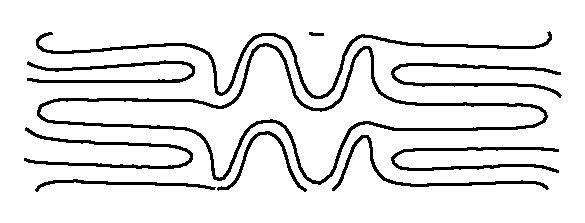
\includegraphics[width=6cm]{images/stent-cell-full}    
    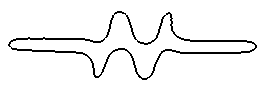
\includegraphics[width=6cm]{images/stent-cell}
  \end{latexonly}
  \begin{htmlonly}
    \htmladdimg{../images/stent-cell-full.png}
    \htmladdimg{../images/stent-cell.png}
  \end{htmlonly}  
  \caption{Intersection of stent cell with plane and inner line of stent cell}
  \label{fig:stent-cell}
\end{figure}

Finally, the \code{length()} function returns the circumference of the cell, which is 9.19 mm.

%%% Local Variables: 
%%% mode: latex
%%% TeX-master: "manual"
%%% End: 
